\documentclass[conference]{IEEEtran}
\IEEEoverridecommandlockouts
% The preceding line is only needed to identify funding in the first footnote. If that is unneeded, please comment it out.
\usepackage{cite}
\ifCLASSOPTIONcompsoc \usepackage[caption=false,font=normalsize,labelfon
t=sf,textfont=sf]{subfig}
\else
\usepackage[caption=false,font=footnotesize]{subfi g}
\fi
\usepackage{amsmath,amssymb,amsfonts}
\usepackage{algorithmic}
\usepackage{graphicx}
\usepackage{textcomp}
\usepackage{xcolor}
\def\BibTeX{{\rm B\kern-.05em{\sc i\kern-.025em b}\kern-.08em
    T\kern-.1667em\lower.7ex\hbox{E}\kern-.125emX}}
\begin{document}

\title{Linear Quadratic Integral Differential Game applied to the Real-time Control of a 3DoF Experimental setup of a Quadrotor\\
% {\footnotesize \textsuperscript{*}Note: Sub-titles are not captured in Xplore and
% should not be used}
% \thanks{In partnership with BaniAsad Industries}
}

\author{\IEEEauthorblockN{Hadi Nobahari}
\IEEEauthorblockA{\textit{Department of Aerospace Engineering} \\
\textit{Sharif University of Technology}\\
Tehran, Iran \\
nobahari@sharif.edu}
\and
\IEEEauthorblockN{Ali BaniAsad}
\IEEEauthorblockA{\textit{Department of Aerospace Engineering} \\
\textit{Sharif University of Technology}\\
Tehran, Iran \\
ali.baniasad@ae.sharif.edu}
\and
\IEEEauthorblockN{Alireza Sharifi}
\IEEEauthorblockA{\textit{Department of Aerospace Engineering} \\
\textit{Sharif University of Technology}\\
Tehran, Iran \\
alireza\_sharifi@ae.sharif.edu}

}

\maketitle

\begin{abstract}
	The accurate attitude control of a quadrotor is necessary, especially when facing disturbance. In this study, a linear quadratic with integral action based on the differential game theory is implemented on a three-degree-of-freedom experimental setup of a quadrotor. For this purpose, first, a continuous state-space model of the quadrotor is derived based on the linearization of the nonlinear equations of motion, and the parameters of the state-space model structure are identified with the experimental results. Then, the attitude control commands of the quadrotor are derived based on two players; one finds the best attitude control command, and the other creates the disturbance by mini-maximizing a quadratic criterion, defined as the sum of outputs plus the weighted control effort and disturbance. The performance of the proposed controller is evaluated in level flight and compared to the linear quadratic regulator controller. Results demonstrate that the proposed approach has an excellent performance in dissipating the disturbances.
\end{abstract}
\begin{IEEEkeywords}
    Linear Quadratic Differential Game, Quadrotor, Real-time, 3DoF Experimental setup, Optimal Control, Robust Control
\end{IEEEkeywords}
\section{Introduction}

\noindent A quadrotor is a type of helicopter with four rotors that plays a significant role in today's society, including research, military, imaging, recreation, and agriculture. The performance of the quadrotor relies on the control system, including attitude, altitude, and position subsystems. In the attitude control of the quadrotor, it is necessary to maintain the attitude outputs, including roll, pitch, and yaw angles of the quadrotor, at the desired level using control commands such as the rotational speed of the rotors, when the disturbances occur suddenly. Therefore, much research is being conducted on the automatic control of the attitudes' quadrotor in facing the disturbance.


     In \cite{PID}, a Proportional Integral Derivative (PID) controller is used to control the attitude of the quadrotor. However, the control objectives have not been effectively achieved with this controllers when the disturbance occurs. To solve this problem the model-based approaches \cite{model_base} are utilized for controller design. These controllers work based on information from the attitude model of the quadrotor and the disturbance to produce the best control command.



     Various model-based controllers can be found within the literature, the most well-known of which are intelligent control, the nonlinear control, robust control, and optimal control to reduce the disturbance effect in the attitude control and provide a faster control algorithm in facing the modeling error. In the intelligent controller category, the artificial intelligence computing approaches like fuzzy logic \cite{fuzzy}, iterative learning \cite{iterative_Learning}, machine learning \cite{machine_learning}, reinforcement learning \cite{Reinforcement_Learning}, and evolutionary computation \cite{Evolutionary} have been utilized to control the attitude of the quadrotor.


     Moreover, nonlinear control methods such as Sliding Mode Control (SMC) \cite{SMC} and Feedback Linearization (FBL) \cite{FBL} have been applied to control the roll, pitch, and yaw angles of the quadrotor. In the optimal controller category, a Linear Quadratic Regulator (LQR) \cite{LQR} and Linear Quadratic Gaussian (LQG) \cite{LQG} have been implemented on the quadrotor based on the minimization of a quadratic criterion, including regulation performance and control effort to provide optimally controlled feedback gains. 


     Linear Quadratic Regulator Differential Game (LQR-DG) control approach \cite{LQDG, robust_LQDG} is a class of optimal and robust controller methods that controls the outputs of a system based on its linear model and mini-maximization of a cost function. This approach has been utilized to stabilize and control various nonlinear and complex systems such as a ship controller \cite{LQDG_ship}. Moreover, in the LQR-DG control method, the control commands are analytically generated based on a pursuit-evasion of two players, one tracks the best control command, and the other creates the disturbance. This is one of the distinctive features of the LQR-DG controller and an important difference from other optimal control methods.


     In this study, an LQR controller method based on the differential game theory, with an integral action called Linear Quadratic Integarl Regulator Differential Game (LQIR-DG) controller, is proposed to generate the most efficient control command for an experimental setup of the quadrotor when facing the disturbance. Since the LQIR-DG is affected by an accurate model of the system, first, the dynamic of the three-degree-of-freedom setup of the quadrotor is modeled. Then, the linear state-space form the quadrotor model is extracted using the linearization of the nonlinear equations of motion to utilize in the proposed control problem. Moreover, the model's parameters are identified and verified against the experimental values. Next, the LQIR-DG technique is applied to the experimental setup of the quadrotor to reduce the effect of disturbance. The performance of the proposed controller is examined in the presence of the disturbance. The results show the successful performance of the LQIR-DG scheme in reducing the disturbance.


     This paper is organized as follows: The problem architecture is defined in section \ref{sec:problem_statement}. In section \ref{sec:modeling}, the dynamics model for the experimental setup of the quadrotor is derived in detail. In section \ref{sec: diff game}, The LQIR-DG architecture is denoted. Numerical results are provided in section \ref{sec:results}. Finally, a conclusion is made in section \ref{sec:conclusion}.
\section{Problem Statement}\label{sec:problem_statement}
\noindent In this section, a nonlinear dynamic is presented for thw experimental setup of the quadrotor, as shown in \figurename{\ref{quadlab}}.
The quadrotor is free to rotate about its roll, pitch, and yaw axes. The Euler angle angles and angular velocities along three orthogonal axes are measured simultaneously using the Attitude and Heading Reference Systems (AHRS). LQIR-DG utilizes these noisy measurements for real-time control of the Euler angles. The block diagram of the proposed controller structure is shown in \figurename{\ref{block_diagram}}.
\vspace{-1cm}
\begin{figure}[!h]
	\vspace{0.1cm}
	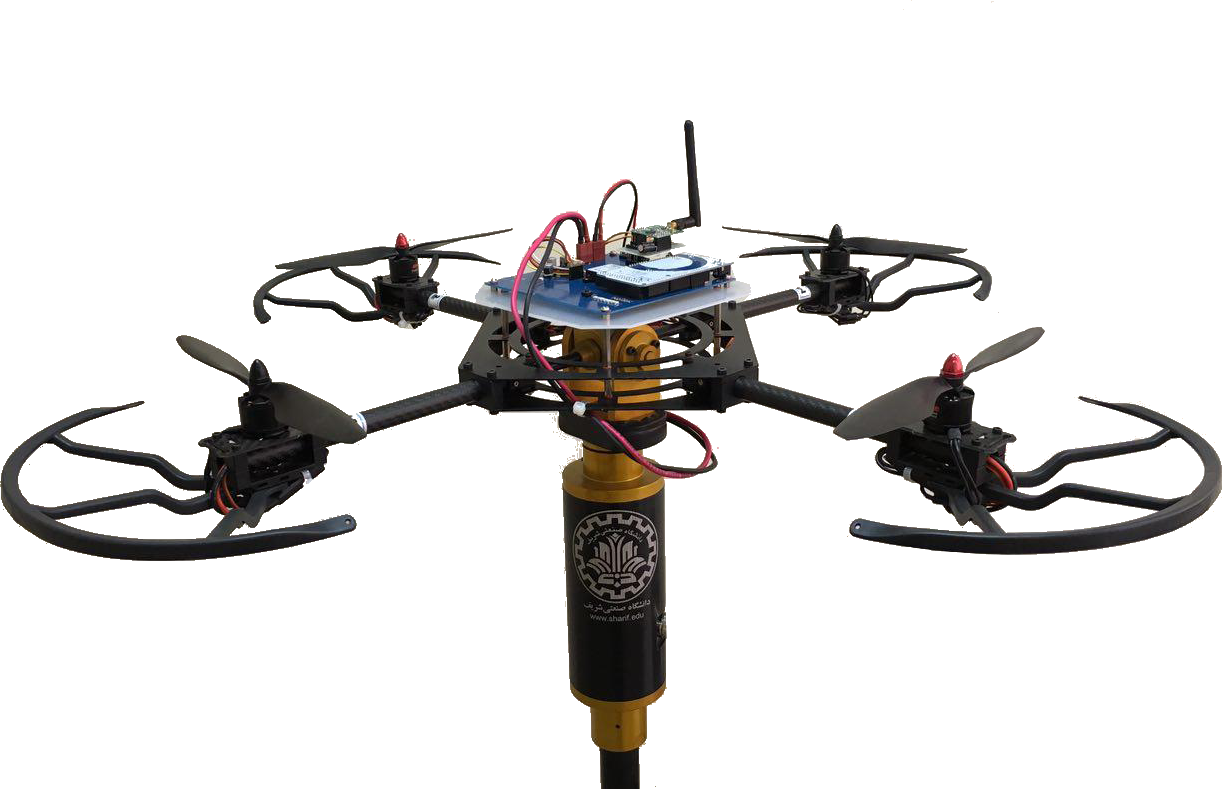
\includegraphics[width=\linewidth]{../Figures/introduction/3DOFQuad.png}
	\centering
	\caption{3DoF experimental setup of a quadrotor}
	\label{quadlab}
\end{figure}
\begin{figure}[!h]
	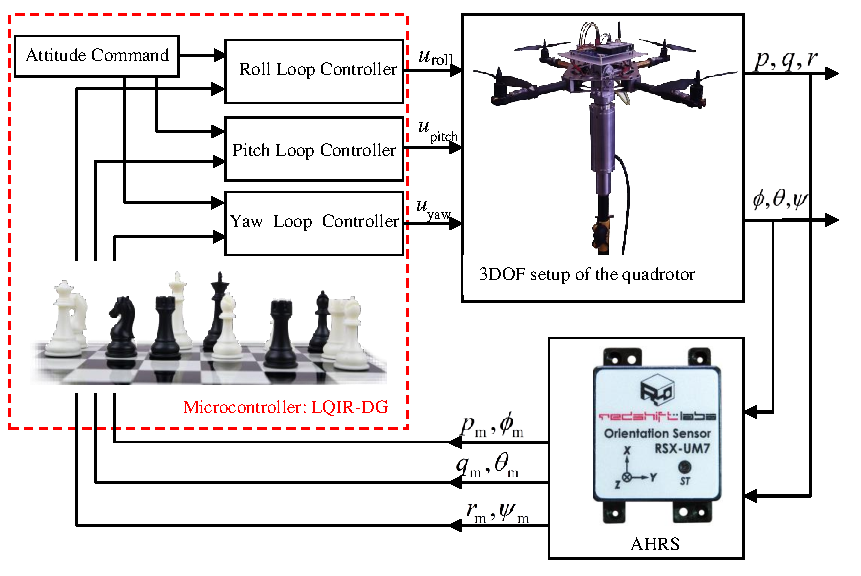
\includegraphics[width=\linewidth]{../Figures/introduction/schematic.pdf}
	\centering
	\caption{Block diagram of the LQIR-DG controller structure}
	\label{block_diagram}
\end{figure}


\section{Modeling of an Experimental Setup of a Quadrotor}\label{sec:modeling}
\noindent Here, the model of the three-degree-of-freedom experimental setup of the quadrotor is presented in details. For this purpose, first, the configuration of the quadrotor is denoted. Then, the nonlinear model of the attitude dynamics is derived to denote the state-space form. Finally, the nonlinear model is linearized to utilize in the control purposes.
\subsection{Configuration of the Quadrotor }
\noindent The schematic of the quadrotor is given in \figurename{\ref{QuadAssum}}. Each rotor is considered a rigid disk is rotating about the axis $z_B$ in the body fixed frame with an angular velocity $\Omega_i$.
Rotors 1 and 3 rotate in the same direction, i.e., counterclockwise, while rotors 2 and 4 rotate in the opposite direction, i.e., clockwise, to cancel yawing moment of the quadrotor.
\vspace{-0.5cm}
\begin{figure}[!h]
	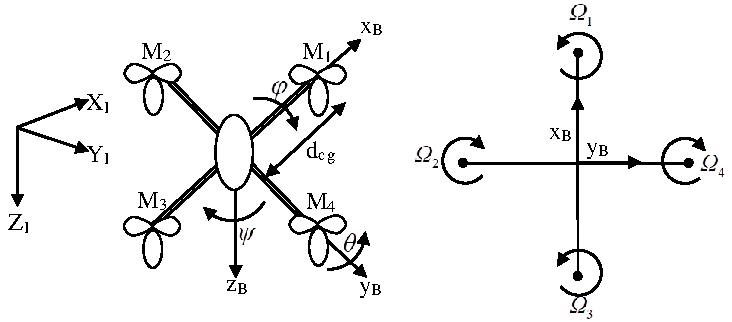
\includegraphics[width=\linewidth]{../Figures/introduction/fig17.pdf}
	\centering
	\caption{Configuration of the quadrotor}
	\label{QuadAssum}
\end{figure}
\subsection{Dynamic Model}
\noindent The dynamic model of the quadrotor, obtained from the Newton-Euler method, is stated as follows \cite{b15}, \cite{b16}:
\begin{equation}
	\begin{split}
		&\dot p = \dfrac{\mathrm{I}_{\text{yy}} - \mathrm{I}_{\text{zz}}}{\mathrm{I}_{\text{xx}}} qr + q \dfrac{\mathrm{I}_{\text{rotor}}}{\mathrm{I}_{\text{xx}}}\Omega_r + \dfrac{u_{\text{roll}}}{\mathrm{I}_{\text{xx}}} + \dfrac{d_{\text{roll}}}{\mathrm{I}_{\text{xx}}}
	\end{split}
\end{equation}
\begin{equation}
	\dot q = \dfrac{\mathrm{I}_{\text{zz}} - \mathrm{I}_{\text{zz}}}{\mathrm{I}_{\text{yy}}} rp + p \dfrac{\mathrm{I}_{\text{rotor}}}{\mathrm{I}_{\text{xx}}}\Omega_r + \dfrac{u_{\text{pitch}}}{\mathrm{I}_{\text{yy}}} + \dfrac{d_{\text{pitch}}}{\mathrm{I}_{\text{yy}}}
\end{equation}
\begin{equation}
	\dot r = \dfrac{\mathrm{I}_{\text{xx}} - \mathrm{I}_{\text{yy}}}{\mathrm{I}_{\text{zz}}} pq  +  \dfrac{u_{\text{yaw}}}{\mathrm{I}_{\text{zz}}} + \dfrac{d_{\text{yaw}}}{\mathrm{I}_{\text{zz}}}
\end{equation}
where $\mathrm{I}_{\text{xx}}$, $\mathrm{I}_{\text{yy}}$, and $\mathrm{I}_{\text{zz}}$ are the principal moment of inertia and $\mathrm{I}_{\text{rotor}}$ is the inertia of a rotor about its axis.. Moreover, $d_{\text{roll}}$, $d_{\text{pitch}}$, and $d_{\text{yaw}}$ are the disturbances, generated in $x_B$, $y_B$ and $z_B$, respectively. $(p, q, r)$ are the angular velocities, and $(\phi, \theta, \psi)$ are roll, pitch, and yaw angles. The relation between the Euler angles rates and the angular body rates are obtained as follows:
\begin{equation}
	\begin{split}
		\dot\phi = p + q\sin(\phi)\cos(\theta) + r\cos(\phi)\tan(\theta)
	\end{split}
\end{equation}
\begin{equation}
	\dot \theta = q\cos(\phi) - r\sin(\phi)
\end{equation}
\begin{equation}
	\dot\psi = (q\sin(\phi) + r\cos(\phi))\sec(\theta) 
\end{equation}
Moreover, $\Omega_r$, called the overall residual propeller angular speed, is computed as
\begin{equation}
	\Omega_r = -\Omega_1 + \Omega_2 - \Omega_3 + \Omega_4
\end{equation}
\subsection{Control Commands}
\noindent The control inputs $u_{\text{roll}}$, $u_{\text{pitch}}$, and $u_{\text{yaw}}$ are roll, pitch, and yaw moments, generated by the propellers, defined as
\begin{equation}
	\begin{split}
		u_{\text{roll}} = \mathrm{b\,d}_{\text{cg}} (\Omega_2^2 - \Omega_4^2)
	\end{split}
\end{equation}
\begin{equation}
	u_{\text{pitch}} = \mathrm{b\,d}_{\text{cg}} (\Omega_1^2 - \Omega_3^2) 
\end{equation}
\begin{equation}
	u_{\text{yaw}} = \mathrm{d} (\Omega_1^2 - \Omega_2^2 + \Omega_3^2 - \Omega_4^2)
\end{equation}

Also, b and d are thrust and drag coefficients, respectively, and $\mathrm{d}_{\text{cg}}$ is the horizontal distance of each rotor from the center of gravity. Therefore, the angular velocity commands are obtained as
\begin{equation}
	\begin{split}
		\Omega_{c, 1}^2 = \Omega_{\text{mean}}^2 + \dfrac{1}{2\mathrm{b\,d}_{\text{cg}}}u_{\text{pitch}} + \dfrac{1}{4d}u_{\text{yaw}} 
	\end{split}
\end{equation}
\begin{equation}
	\Omega_{c, 2}^2 = \Omega_{\text{mean}}^2 + \dfrac{1}{2\mathrm{b\,d}_{\text{cg}}}u_{\text{roll}} - \dfrac{1}{4d}u_{\text{yaw}}
\end{equation}
\begin{equation}
	\Omega_{c, 3}^2 = \Omega_{\text{mean}}^2 - \dfrac{1}{2\mathrm{b\,d}_{\text{cg}}}u_{\text{pitch}} + \dfrac{1}{4d}u_{\text{yaw}} 
\end{equation}
\begin{equation}
\Omega_{c, 4}^2 = \Omega_{\text{mean}}^2 - \dfrac{1}{2\mathrm{b\,d}_{\text{cg}}}u_{\text{roll}} - \dfrac{1}{4d}u_{\text{yaw}}
\end{equation}
where $\Omega_{\text{mean}}$ is the average angular velocity of the rotors.
\subsection{State-Space Form}
\noindent Here, the state-space model of the experimental setup of the quadrotor is presented for the control purposes. by defining $x_1 = p$, $x_2 = q$, $x_3 = r$, $x_4 = \phi$, $x_5 = \theta$, and $x_6 = \psi$; the model of the experimental setup in state-space form are expressed as
\begin{equation}\label{eq:diffeq}
	\begin{split}
		\dot x_1 = \dfrac{\mathrm{I}_{\text{yy}} - \mathrm{I}_{\text{zz}}}{\mathrm{I}_{\text{xx}}} x_2 x_3 + x_2 \dfrac{\mathrm{I}_{\text{rotor}}}{\mathrm{I}_{\text{xx}}}\Omega_r + \dfrac{u_{\text{roll}}}{\mathrm{I}_{\text{xx}}} + \dfrac{d_{\text{roll}}}{\mathrm{I}_{\text{xx}}} 
	\end{split}
\end{equation}
\begin{equation}
	\dot x_2 = \dfrac{\mathrm{I}_{\text{zz}} - \mathrm{I}_{\text{zz}}}{\mathrm{I}_{\text{yy}}} x_1 x_3 - x_1 \dfrac{\mathrm{I}_{\text{rotor}}}{\mathrm{I}_{\text{xx}}}\Omega_r + \dfrac{u_{\text{pitch}}}{\mathrm{I}_{\text{yy}}} + \dfrac{d_{\text{pitch}}}{\mathrm{I}_{\text{yy}}}
\end{equation}
\begin{equation}
	\dot x_3 = \dfrac{\mathrm{I}_{\text{xx}} - \mathrm{I}_{\text{yy}}}{\mathrm{I}_{\text{zz}}} x_1 x_2 + \dfrac{u_{\text{yaw}}}{\mathrm{I}_{\text{zz}}} + \dfrac{d_{\text{yaw}}}{\mathrm{I}_{\text{zz}}}
\end{equation}
\begin{equation}
	\dot x_4 = x_1 + x_2\sin(x_4)\cos(x_5) + x_3\cos(x_4)\tan(x_5)
\end{equation}
\begin{equation}
	\dot x_5 = x_2\cos(x_4) - x_3\sin(x_4)
\end{equation}
\begin{equation}\label{eq:diffeq-end}
	\dot x_6 = (x_2\sin(x_4) + x_3\cos(x_4))\sec(x_5)
\end{equation}
The measurement model is written as
\begin{equation}
	\begin{split}
		\boldsymbol{\mathrm{z}} &= \begin{bmatrix}
			p_m & q_m & r_m & \phi_m & \theta_m & \psi_m
		\end{bmatrix}^\mathrm{T}
		\\
		& = \begin{bmatrix}
			x_1 & x_2 & x_3 & x_4 & x_5 & x_6
		\end{bmatrix}^\mathrm{T}
	\end{split}
\end{equation}

\subsection{Linear Model}
\noindent The continuous-time linear model is utilized to drive the control commands on the quadrotor. The linear state-space model is denoted as
\begin{equation}\label{eq:linear}
	\boldsymbol{\dot{\mathrm{x}}}(t) = \boldsymbol{\mathrm{Ax}}(t) + \boldsymbol{\mathrm{Bu}}(t) + \boldsymbol{\mathrm{B_{d}d}}(t)
\end{equation}
where $\boldsymbol{\mathrm{d}}$ is the disturbance. $\boldsymbol{\mathrm{A}}$, $\boldsymbol{\mathrm{B}}$, and $\boldsymbol{\mathrm{B_d}}$ are the system input and disturbance matrices, respectively. Moreover, the measurements equation is stated as
\begin{equation}
	\boldsymbol{{\mathrm{z}}}(t) = \boldsymbol{\mathrm{x}}(t)
\end{equation}


According to Eqs.\eqref{eq:diffeq}-\eqref{eq:diffeq-end}, the linear dynamic model around the equilibrium points $(\boldsymbol{{\mathrm{x}}}_e\!=\!0 \text{ and } \boldsymbol{{\mathrm{u}}}_e\!=\!0)$ of the quadrotor setup is denoted as
\begin{equation}
	\begin{split}
		\boldsymbol{{\mathrm{\dot x}}} = \begin{bmatrix}
			\boldsymbol{{\mathrm{\dot x_{\text{roll}}}}}\\
			\boldsymbol{{\mathrm{\dot x_{\text{pitch}}}}}\\
			\boldsymbol{{\mathrm{\dot x_{\text{yaw}}}}}
		\end{bmatrix} &= \begin{bmatrix}
			\boldsymbol{{\mathrm{A_{\text{roll}}}}} & \boldsymbol{0} & \boldsymbol{0}\\
			\boldsymbol{0} & \boldsymbol{{\mathrm{A_{\text{pitch}}}}} & \boldsymbol{0} \\
			\boldsymbol{0} & \boldsymbol{0} & \boldsymbol{{\mathrm{A_{\text{yaw}}}}}
		\end{bmatrix} \begin{bmatrix}
			\boldsymbol{{\mathrm{x_{\text{roll}}}}}\\
			\boldsymbol{{\mathrm{x_{\text{pitch}}}}}\\
			\boldsymbol{{\mathrm{x_{\text{yaw}}}}}
		\end{bmatrix}
		\\[1em]
		& + \begin{bmatrix}
			\boldsymbol{{\mathrm{B_{\text{roll}}}}} & \boldsymbol{0} & \boldsymbol{0}\\
			\boldsymbol{0} & \boldsymbol{{\mathrm{B_{\text{pitch}}}}} & \boldsymbol{0} \\
			\boldsymbol{0} & \boldsymbol{0} & \boldsymbol{{\mathrm{B_{\text{yaw}}}}}
		\end{bmatrix}
		\begin{bmatrix}
			\boldsymbol{{\mathrm{u_{\text{roll}}}}}\\
			\boldsymbol{{\mathrm{u_{\text{pitch}}}}}\\
			\boldsymbol{{\mathrm{u_{\text{yaw}}}}}
		\end{bmatrix}\\[1em]
		& + \begin{bmatrix}
			\boldsymbol{{\mathrm{B_{\text{roll}}}}} & \boldsymbol{0} & \boldsymbol{0}\\
			\boldsymbol{0} & \boldsymbol{{\mathrm{B_{\text{pitch}}}}} & \boldsymbol{0} \\
			\boldsymbol{0} & \boldsymbol{0} & \boldsymbol{{\mathrm{B_{\text{yaw}}}}}
		\end{bmatrix} \begin{bmatrix}
			\boldsymbol{{\mathrm{d_{\text{roll}}}}}\\
			\boldsymbol{{\mathrm{d_{\text{pitch}}}}}\\
			\boldsymbol{{\mathrm{d_{\text{yaw}}}}}
		\end{bmatrix}
	\end{split}
\end{equation}
where $\boldsymbol{\mathrm{x}}_{\text{roll}} = \begin{bmatrix}
	p & \phi
\end{bmatrix}^\mathrm{T}$, $\boldsymbol{\mathrm{x}}_{\text{pitch}} = \begin{bmatrix}
	q & \theta \end{bmatrix}^\mathrm{T}$, and $\boldsymbol{\mathrm{x}}_{\text{yaw}} = \begin{bmatrix}
	r & \psi
\end{bmatrix}^\mathrm{T}$.


Moreover, the state and input matrices are presented as
\begin{equation}
	\begin{split}
		\boldsymbol{\mathrm{A}}_{\text{roll}}  =\boldsymbol{\mathrm{A}}_{\text{pitch}}  = \boldsymbol{\mathrm{A}}_{\text{yaw}}  = \begin{bmatrix}
			0 & 0\\
			1 & 0
		\end{bmatrix}
	\end{split}
\end{equation}

\begin{equation}
	\begin{split}
		\boldsymbol{\mathrm{B}}_{\text{roll}}  = \begin{bmatrix}
			\dfrac{1}{\mathrm{I}_{\text{xx}}}
			\\[1em]
			0
		\end{bmatrix};~ \boldsymbol{\mathrm{B}}_{\text{pitch}}  = \begin{bmatrix}
			\dfrac{1}{\mathrm{I}_{\text{yy}}}
			\\[1em]
			0
		\end{bmatrix};~ \boldsymbol{\mathrm{B}}_{\text{yaw}}  = \begin{bmatrix}
			\dfrac{1}{\mathrm{I}_{\text{zz}}}
			\\[1em]
			0
		\end{bmatrix}
	\end{split}
\end{equation}




\section{Formulation of the Controller Design}\label{sec: diff game}

\noindent In the LQIR-DG controller structure, an integral action is added to the LQR-DG controller to cancel the steady-state errors for reference tracking. For this purpose, first, the augmented state space of the linear quadrotor model is defined to utilize in the controller architecture. Then, the LQR-DG controller design procedure is presented to generate the best control commands for the experimental setup of the quadrotor.

\subsection{Augmented State Space Formulation}
\noindent To add the integral action to the controller structure, the augmented states are defined as follows:
\begin{equation}\label{lqidg_x}
    \boldsymbol{\mathrm{x_{a_i}}} = \begin{bmatrix}
        \boldsymbol{\mathrm{x_i}} &
        \displaystyle \int \boldsymbol{\mathrm{x_i}}
    \end{bmatrix}^\mathrm{T}
\end{equation}
where $i$ = roll, pitch, and yaw.
Then, the model of the quadrotor dynamics, denoted by Eq.\eqref{eq:linear}, is represented in the augmented state-space model as

\begin{equation}\label{systemlqidg}
	\begin{split}
		\boldsymbol{\dot{\mathrm{x}}_a}(t) &= \boldsymbol{\mathrm{A_ax_a}}(t) + \boldsymbol{\mathrm{B_{{a}}u}}(t) + \boldsymbol{\mathrm{B_{{d_a}}d}}(t)%, \quad \boldsymbol{x}(0) = 
	\end{split}
\end{equation}
where matrices $\boldsymbol{\mathrm{A_a}}$ and $\boldsymbol{\mathrm{B_a}}$ are defined as follows:

\begin{equation}
	\boldsymbol{\mathrm{A_a}} = \begin{bmatrix}
		\boldsymbol{\mathrm{A}} & \boldsymbol{0}\\
		\boldsymbol{\mathrm{I}} & \boldsymbol{0}
	\end{bmatrix}
\end{equation}
\begin{equation}
	\boldsymbol{\mathrm{B_a}} = \boldsymbol{\mathrm{B_{{d_a}}}} = \begin{bmatrix}
		\boldsymbol{\mathrm{B}}\\
		\boldsymbol{0}
	\end{bmatrix}
\end{equation}
In the above equation $\boldsymbol{\mathrm{I}}$ denotes the identity matrix.
\subsection{LQIR-DG Controller Method}
\noindent The LQIR-DG controller is an optimal and robust method based on the differential game theory. This controller consists of two essential players: one finds the best control command, and the other creates the worst disturbance. 
For this purpose, the first player tries to minimize a cost function; while the second is assumed to maximize it. Therefore, the quadratic cost function equation is denoted using min-max operators as follows:
\begin{equation}
	    \begin{split}
		&\min_{u} \max_{d} J(\boldsymbol{\mathrm{x_{a_i}}}, {u_i}, {d_i}) = J(\boldsymbol{\mathrm{x_{a_i}}}, {u^*_i}, {d^*_i})= \\ & ~~\min_{u} \max_{d}
         \int_{0}^{\mathrm{t_f}}\biggl (\boldsymbol{\mathrm{x^\mathrm{T}_{a_i}}}  \boldsymbol{\mathrm{Q_i}} \boldsymbol{\mathrm{x_{a_i}}}+
        {{u^\mathrm{T}_i}}  {{R}} {{u_i}}-
        {{d^\mathrm{T}_{i}}} {{ R_{d} d_{i}}}
        \biggl )\mathrm{d}t
    \end{split}
\end{equation}
where $\mathrm{t_f}$ is the final time. Moreover, ${{ R}}$ and ${{R_{d}}}$ are symmetric nonnegative definite matrices and $\boldsymbol{\mathrm{Q_i}} $ is a symmetric positive definite matrix. To solve this problem, connections between the general optimal problem and the LQIR problem are considered \cite{LQDG} and consequently the optimum control effort is computed for the each control loop as follows:
\begin{equation}
	\begin{split}
		{{u_i}}(t) = -\boldsymbol{{\mathrm{K}}_{i}}(t) \boldsymbol{{\mathrm{x_{a_i}}}}(t)
	\end{split}
\end{equation}
\begin{equation}
	{{d_i}}(t) = \boldsymbol{{\mathrm{K}}_{i}}(t)\boldsymbol{{\mathrm{x_{a_i}}}}(t)
\end{equation}
where $\boldsymbol{{\mathrm{K_i}}}$ and $\boldsymbol{{\mathrm{K_{d_i}}}}$ are a time varying gain, given by
\begin{equation}
	\boldsymbol{{\mathrm{K_i}}} = {{{R}}^{-1}}\boldsymbol{{\mathrm{B}_{a_i}^\mathrm{T}}}\boldsymbol{{\mathrm{P}}_{a_i}}(t)
\end{equation}
\begin{equation}
	\boldsymbol{{\mathrm{K_{d_i}}}} = {{{R}}^{-1}_{d}}\boldsymbol{{\mathrm{B}_{a_{d_i}}^\mathrm{T}}}\boldsymbol{{\mathrm{P}}_{a_{d_i}}}(t)
\end{equation}
where $\boldsymbol{{\mathrm{P}}_{a_i}}(t)$ and $\boldsymbol{{\mathrm{P}}_{a_{d_i}}}(t)$ satisfy
\begin{equation}\label{coupled_riccatti_LQIDG}
        \begin{split}
            \boldsymbol{\dot{\mathrm{P}}_{a_i}}&(t) = -\boldsymbol{\mathrm{A^\mathrm{T}_a}}\boldsymbol{\mathrm{P_{a_i}}}(t) - \boldsymbol{\mathrm{P_{a_i}}}(t)\boldsymbol{\mathrm{A_a}} - \boldsymbol{\mathrm{Q_i}} +\\ &\boldsymbol{\mathrm{P_{a_i}}}(t)\boldsymbol{\mathrm{S_{a_i}}}(t)\boldsymbol{\mathrm{P_{a_i}}}(t) + \boldsymbol{\mathrm{P_{a_i}}}(t)\boldsymbol{\mathrm{S_{a_{d_i}}}}(t)\boldsymbol{\mathrm{P_{a_{d_i}}}}(t)
        \end{split}
	\end{equation}
	\begin{equation}
        \begin{split}
            \boldsymbol{\dot{\mathrm{P}}_{a_{d_i}}}&(t) = -\boldsymbol{\mathrm{A^\mathrm{T}_a}}\boldsymbol{\mathrm{P_{a_{d_i}}}}(t) - \boldsymbol{\mathrm{P_{a_{d_i}}}}(t)\boldsymbol{\mathrm{A_a}} - \boldsymbol{\mathrm{Q_{i}}} +\\ &\boldsymbol{\mathrm{P_{a_{d_i}}}}(t)\boldsymbol{\mathrm{S_{a_{d_i}}}}(t)\boldsymbol{\mathrm{P_{a_{d_i}}}}(t) + \boldsymbol{\mathrm{P_{a_{d_i}}}}(t)\boldsymbol{\mathrm{S_{a_i}}}(t)\boldsymbol{\mathrm{P_{a_i}}}(t)
        \end{split}
\end{equation}
where $\boldsymbol{\mathrm{S_{a_i}}} = \boldsymbol{\mathrm{B_{a_i}}}R^{-1}\boldsymbol{\mathrm{B}^\mathrm{T}_{a_i}}$ and $\boldsymbol{\mathrm{S_{a_{d_i}}}} = \boldsymbol{\mathrm{B}_{a_{d_i}}}R_{d}^{-1}\boldsymbol{\mathrm{B}^\mathrm{T}_{a_{d_i}}}$.
In this study, the steady-state values of the above equations $(\boldsymbol{{\mathrm{P}}} \text{ as } \mathrm{t_f} \to \infty)$ are utilized to generate a feedback control law.








\section{Result and Discussion}\label{sec:results}


\noindent Here, the results of the LQIR-DG controller method are devoted to the control loops of the roll, pitch, and yaw of the experimental setup of the quadrotor. First, the controller parameters are tuned using the results of numerical simulations. Moreover, the performance of the LQIR-DG controller is compared to an LQR control strategy. The parameters of the quadrotor are shown in table \ref{tab:parameters}.
Moreover, the parameters of LQIR-DG controller weight are denoted in table \ref{tab:control weight_new}.
\begin{table}[!h]
	\renewcommand{\arraystretch}{1.3}
	\caption{The Parameter of the Quadrotor}
	\begin{center}
	\begin{tabular}{c c c}
	\hline
	\textbf{Parameter} & \textbf{\textit{Value}}& \textbf{\textit{Unit}} \\
	\hline
	$\mathrm{I}_{\text{xx}}$ & $0.02839$ & $kg.m^2$ \\
	$\mathrm{I}_{\text{yy}}$  & $0.03066$ & $kg.m^2$\\
	$\mathrm{I}_{\text{zz}}$  & $0.0439$ & $kg.m^2$ \\
	$\mathrm{I}_{\text{rotor}}$  & $4.4398\times 10^{-5}$ & $kg.m^2$\\
	$\mathrm{b}$  & $3.13\times10^{-5}$ & $1$ \\
	$\mathrm{d}$  & $3.2\times10^{-6}$ & $1$\\
	$\Omega_{\text{mean}}$ & $3000$ & rpm \\
	$\mathrm{d}_{\text{cg}}$  & $0.2$ & $m$\\
	\hline
	\end{tabular}
	\label{tab:parameters}
	\end{center}
\end{table}


\begin{table}[!h]
	\renewcommand{\arraystretch}{1.3}
	\caption{The Parameters of the LQIR-DG Controller}
	\begin{center}
	\begin{tabular}{c c c}
	\hline
	\textbf{Control Loop} & \textbf{\textit{Weight}}& \textbf{\textit{Value}} \\
	\hline
	Roll & 
	$\boldsymbol{{\mathrm{Q_{\text{roll}}}}}$ & diag([$7.91$, $0.01$, $631.85$, $214.28$])\\
	Pitch & 
	$\boldsymbol{{\mathrm{Q_{\text{pitch}}}}}$ & diag([$9853.09$, $0.12$, $0.01$, $873.93$])\\
	Yaw & 
	$\boldsymbol{{\mathrm{Q_{\text{yaw}}}}}$ & diag([$1.81e\!-\!4$, $4.5e\!-\!4$, $3e\!-\!6$, $1.7e\!-\!5$])\\
	-& $R$ & 1\\
	-& $R_{d}$ & 1.2577\\
	% $4.5e\!-\!5$])\\
	%  & 
	%  \\
	% Yaw & 
	% $3e\!-\!6$ & $1.7e\!-\!5$ & $1.81e\!-\!4$ &
	% $4.5e\!-\!5$ \\
	\hline
	\end{tabular}
	\end{center}
	\label{tab:control weight_new}
\end{table}


\subsection{Performance of the LQIR-DG Controller}

\noindent The performance of the LQIR-DG controller is evaluated in Figure 8. The desired and actual outputs, including the roll, pitch, and yaw angles, are compared in \figurename{\ref{fig:result}}. The desired scenario of the simulator is considered as a level flight. These figures show that the attitude outputs of the quadrotor converge to the desired values in less than three seconds. Moreover, \figurename{\ref{fig:omega}} show the angular velocity command of the quadrotor, 
respectively. These results illustrate that the LQIR-DG approach appropriately controls the attitude of the experimental setup of the quadrotor.


\begin{figure}[!h]
	\centering
	\subfloat[]{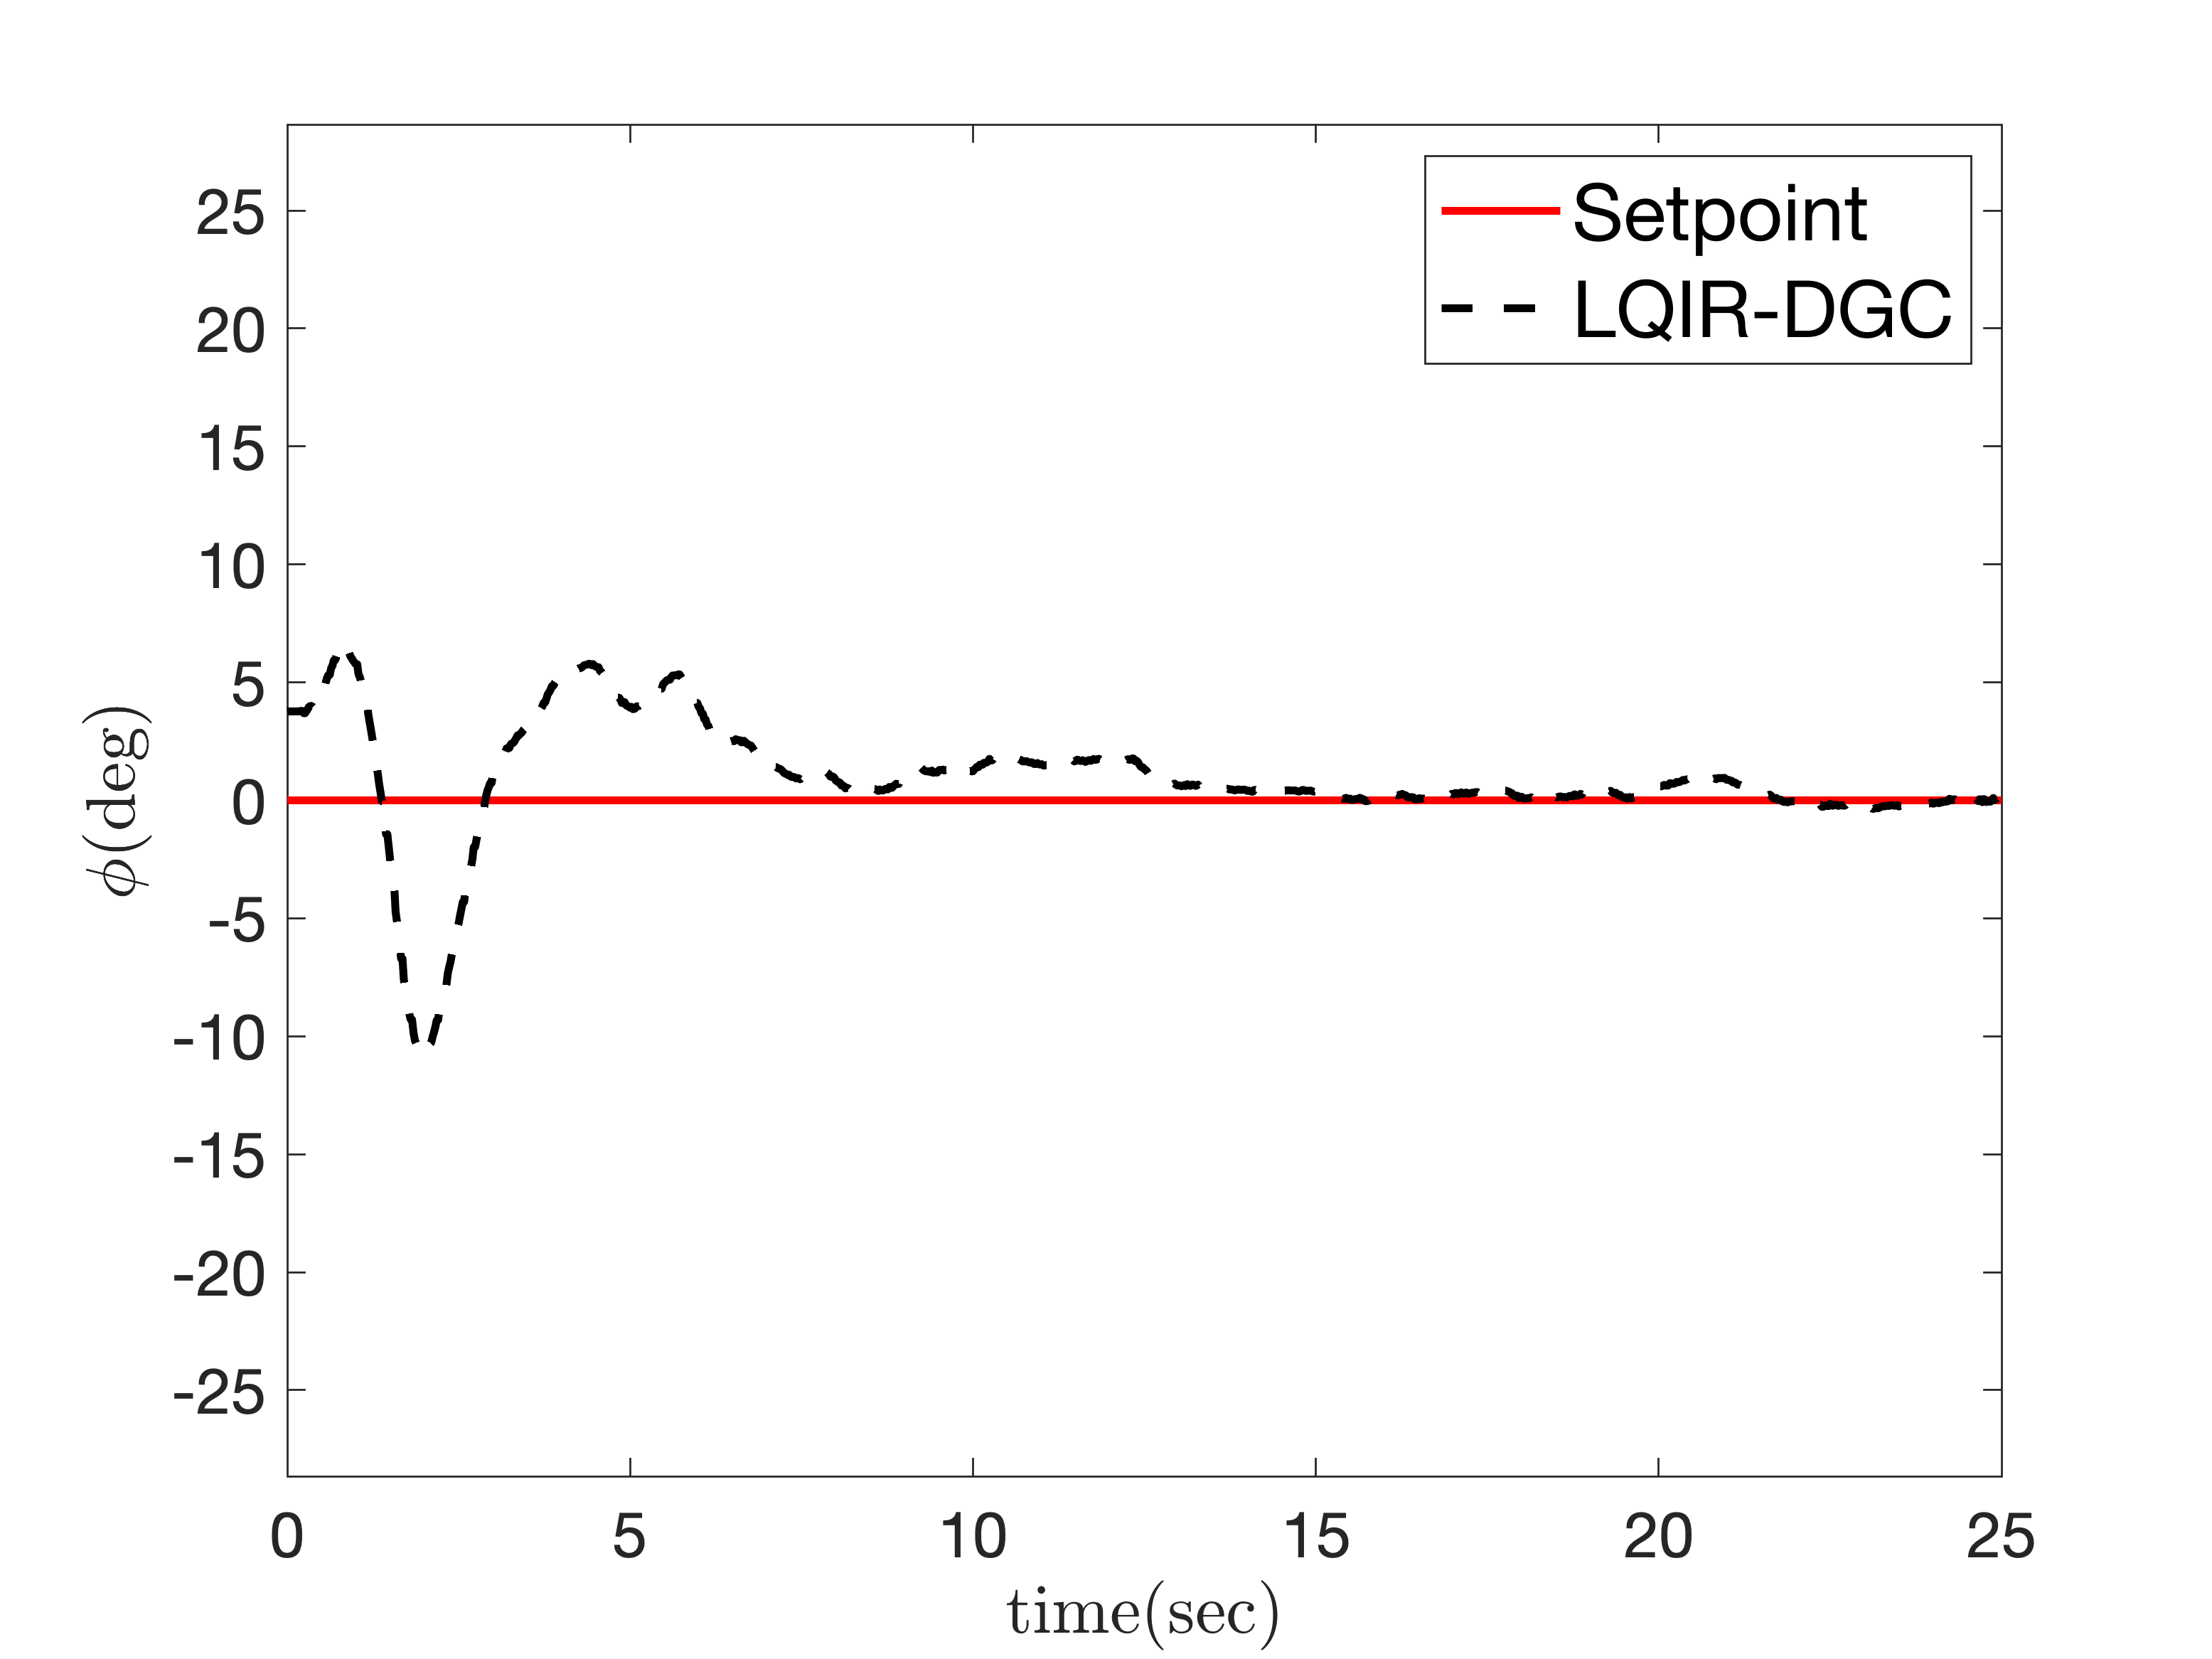
\includegraphics[width=.49\linewidth]{../Figures/Calibration/LQIDG/3DOF/lqidg_roll.png}\label{fig:roll}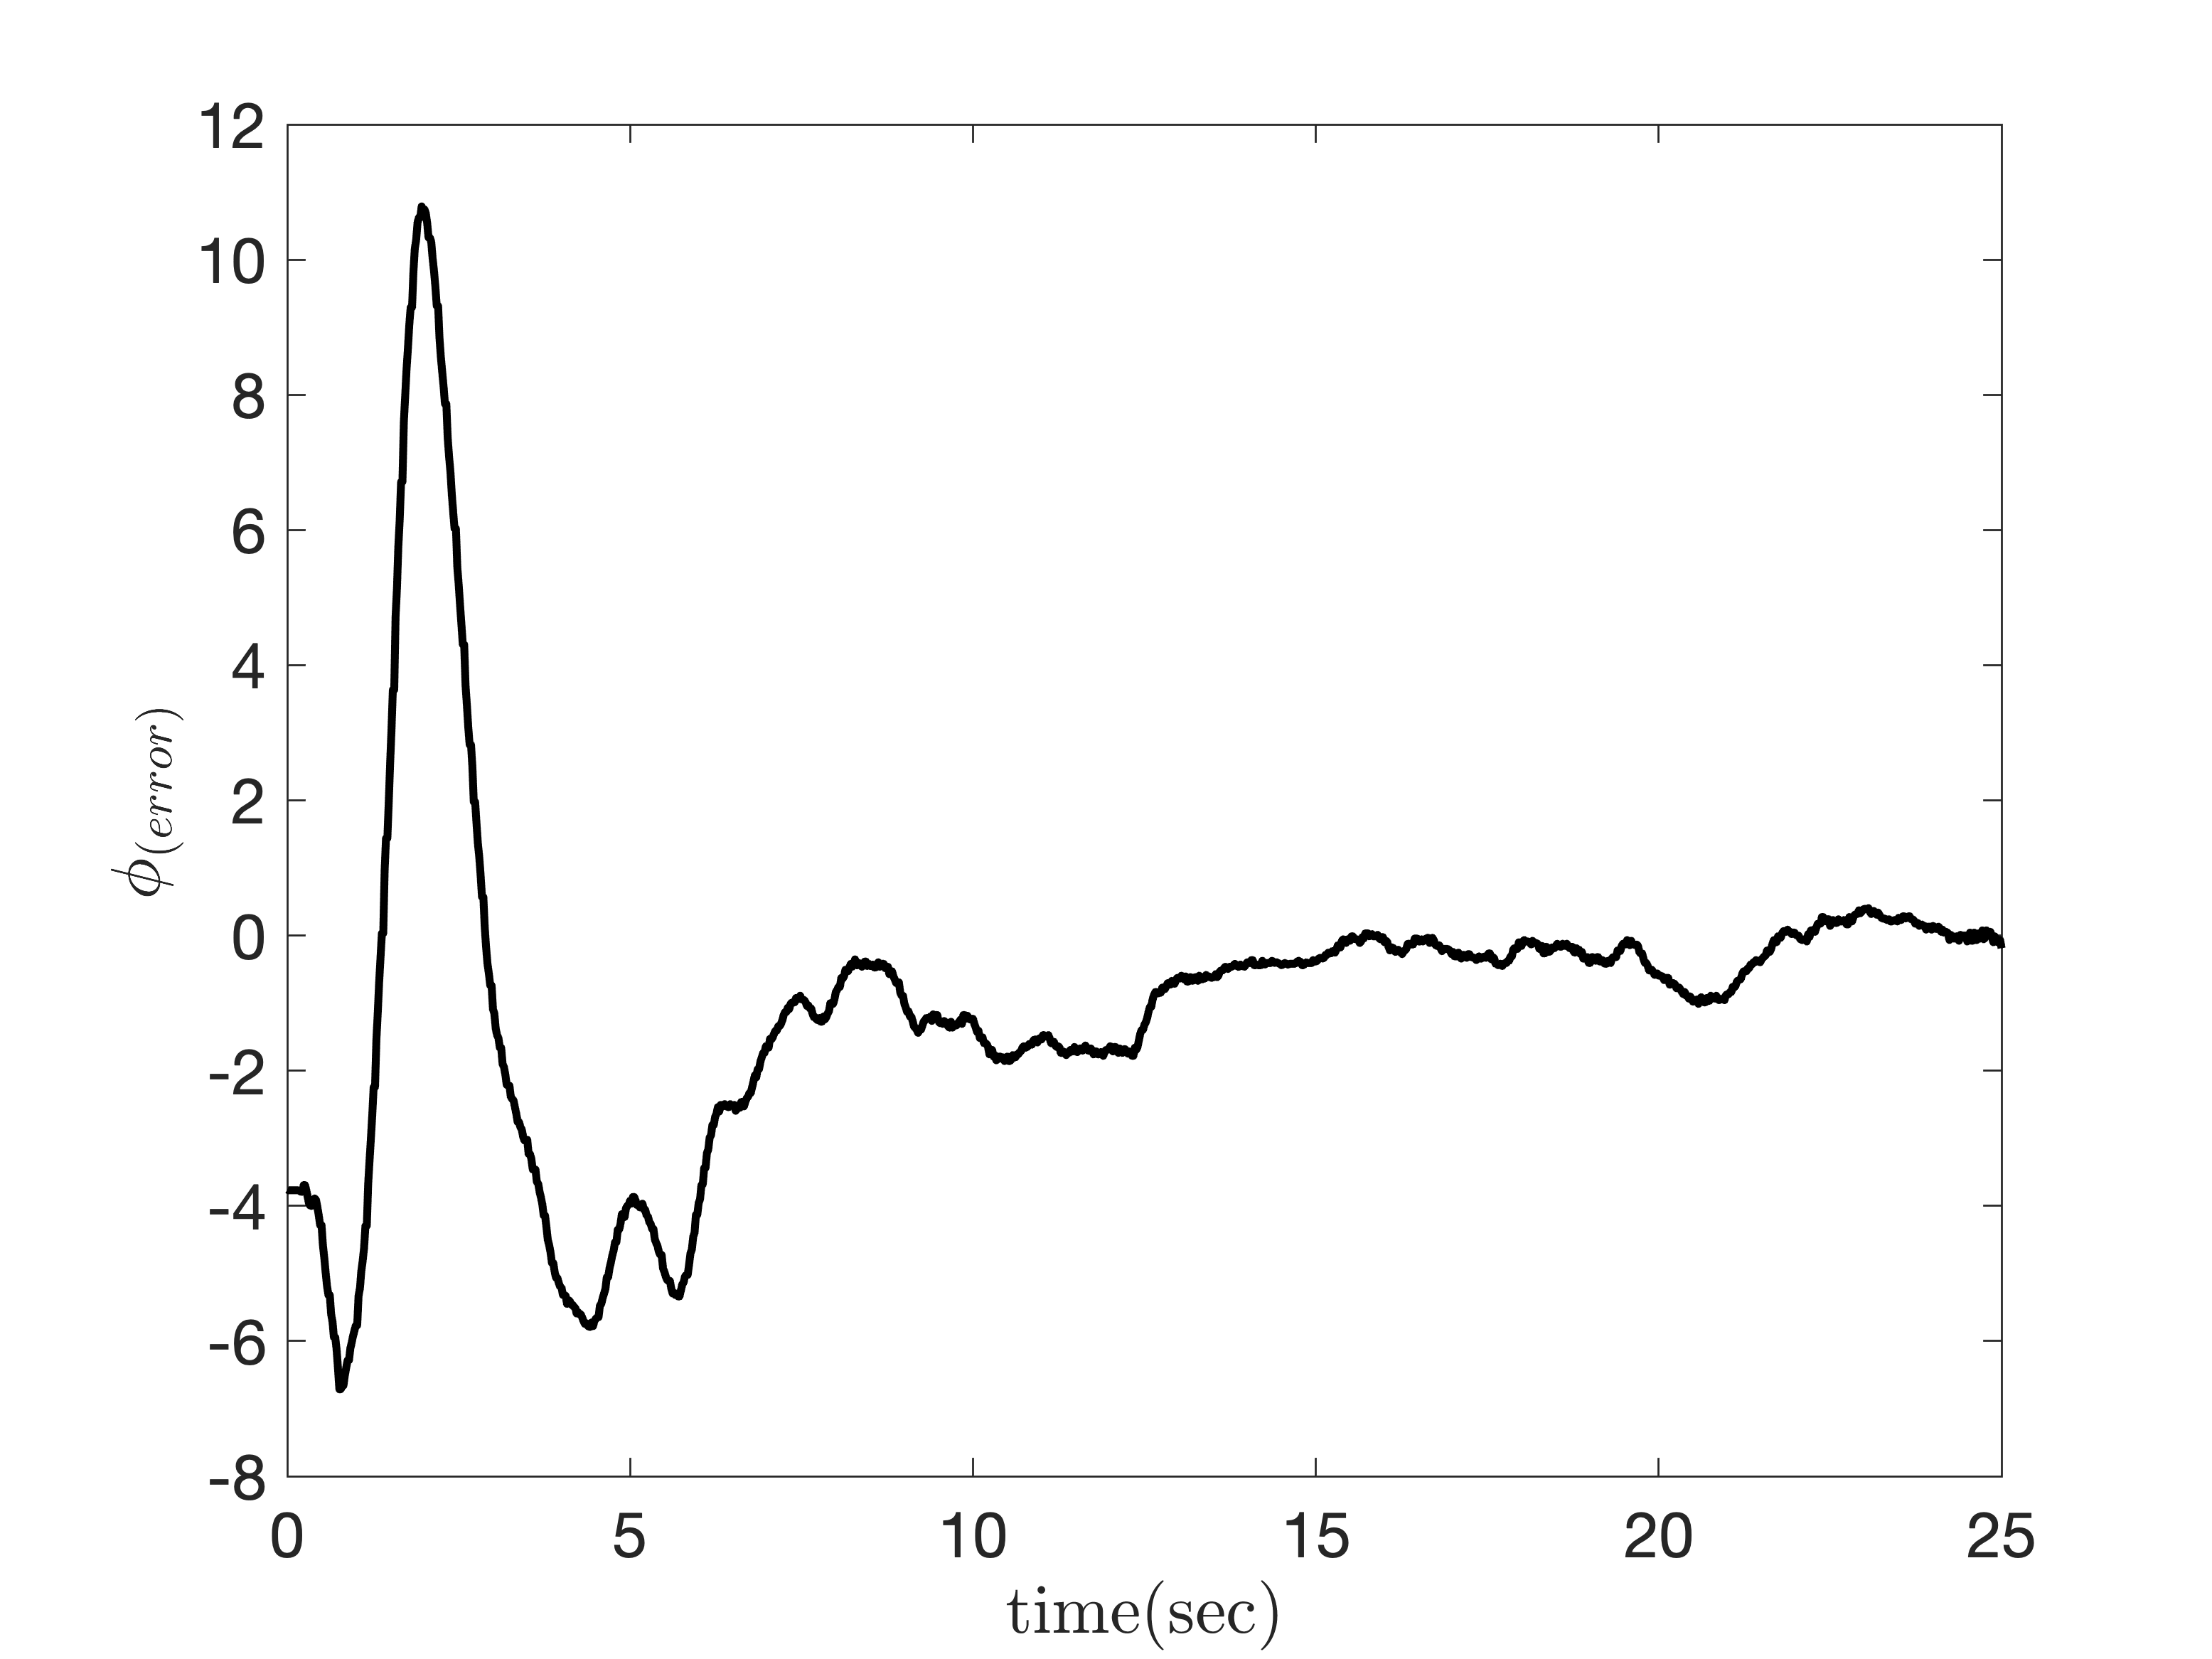
\includegraphics[width=.49\linewidth]{../Figures/Calibration/LQIDG/3DOF/lqidg_roll_e.png}
	}
	% \subfloat{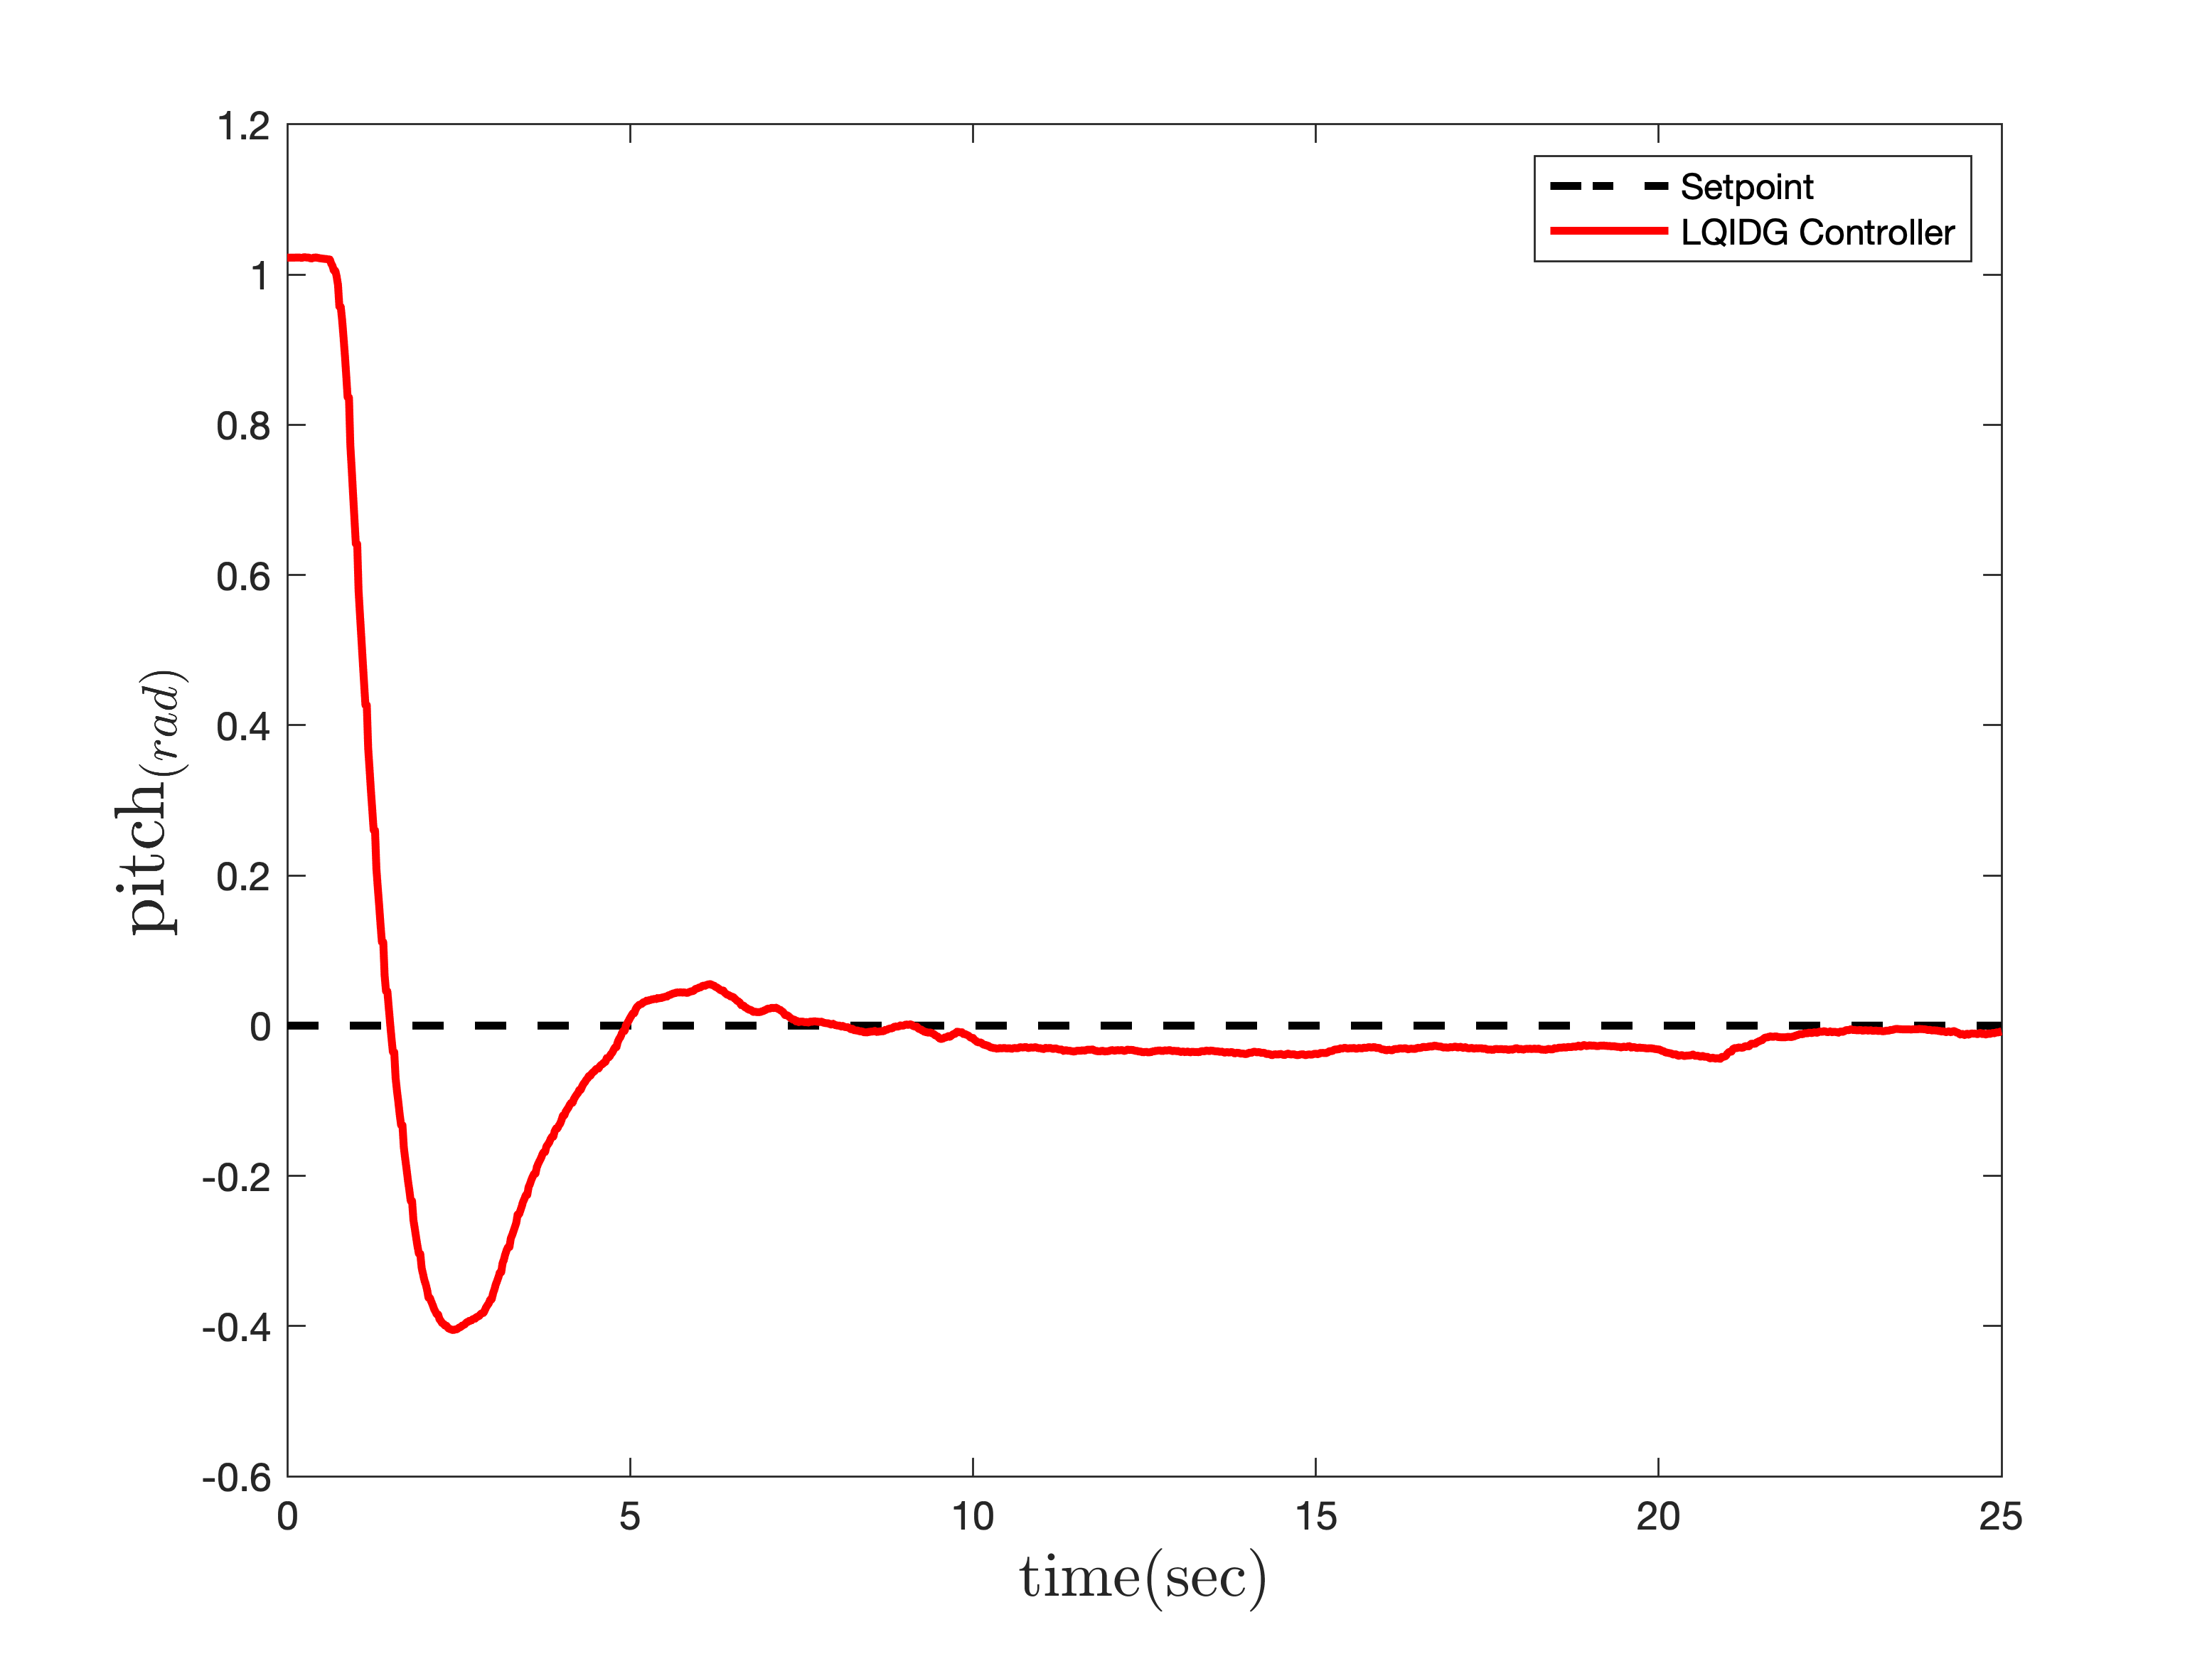
\includegraphics[width=.49\linewidth]{../Figures/Calibration/LQIDG/3DOF/lqidg_pitch.png}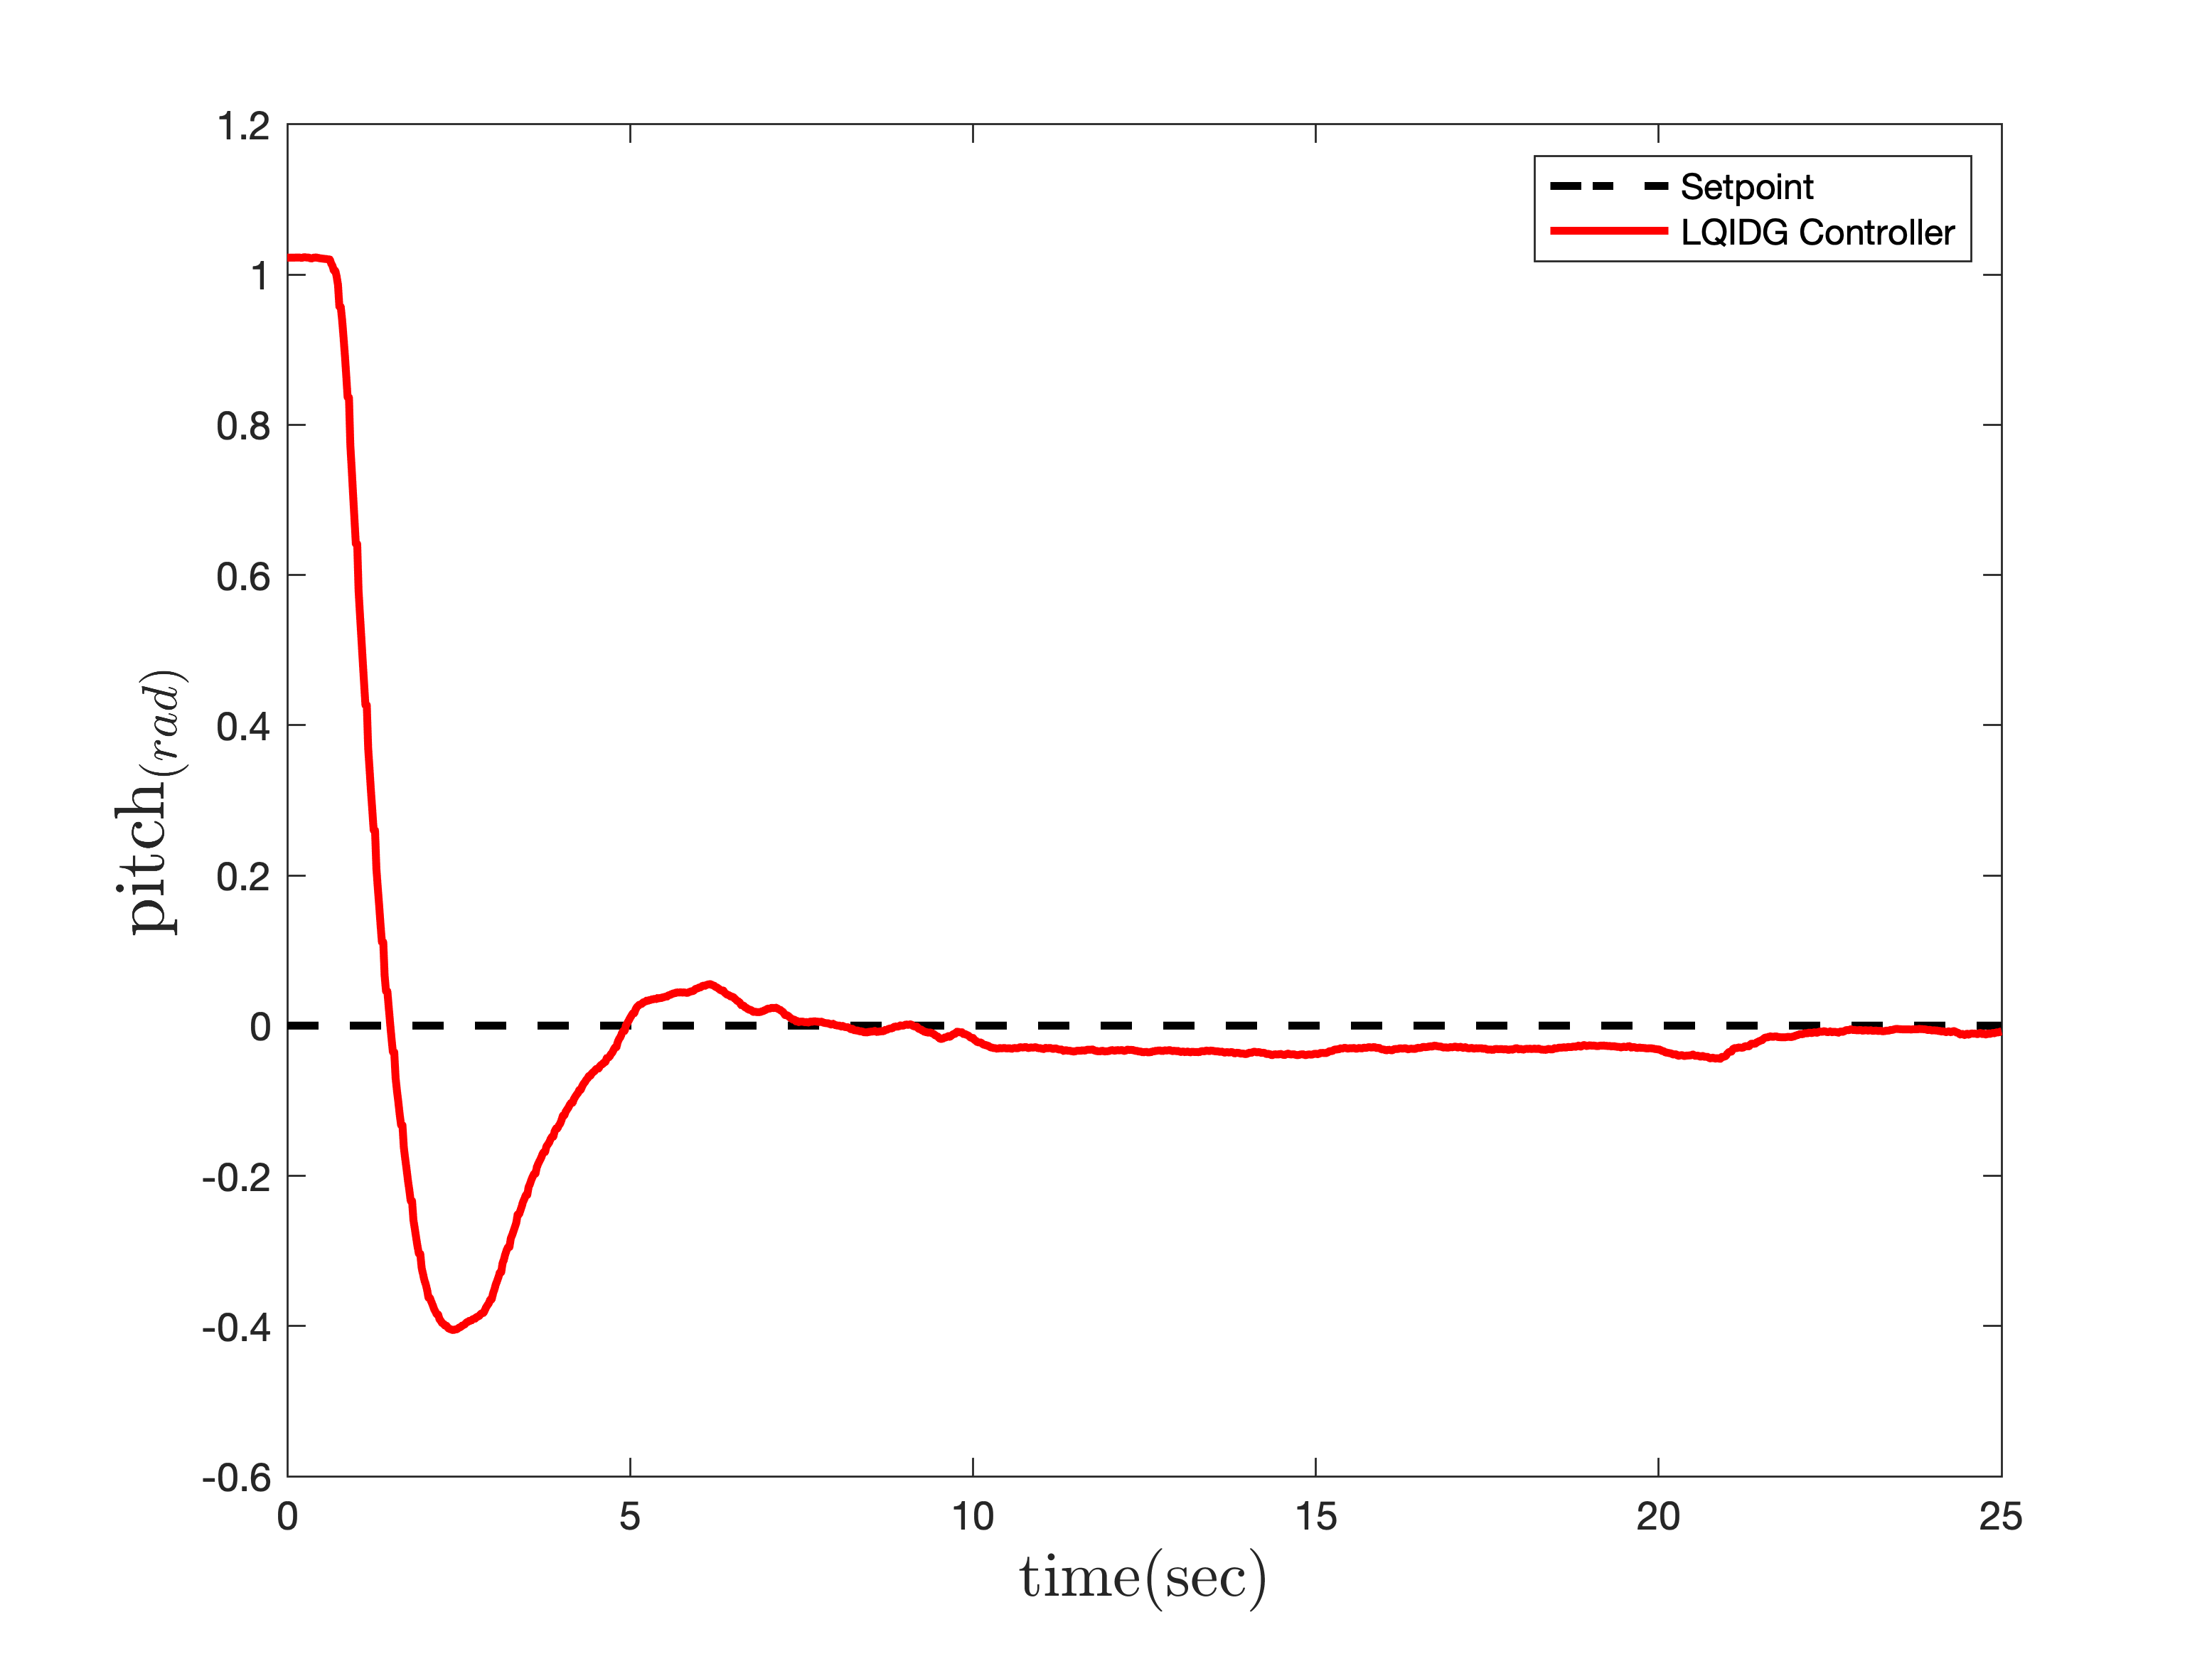
\includegraphics[width=.49\linewidth]{../Figures/Calibration/LQIDG/3DOF/lqidg_pitch.png}
	% }
	\hfil
	\subfloat[]{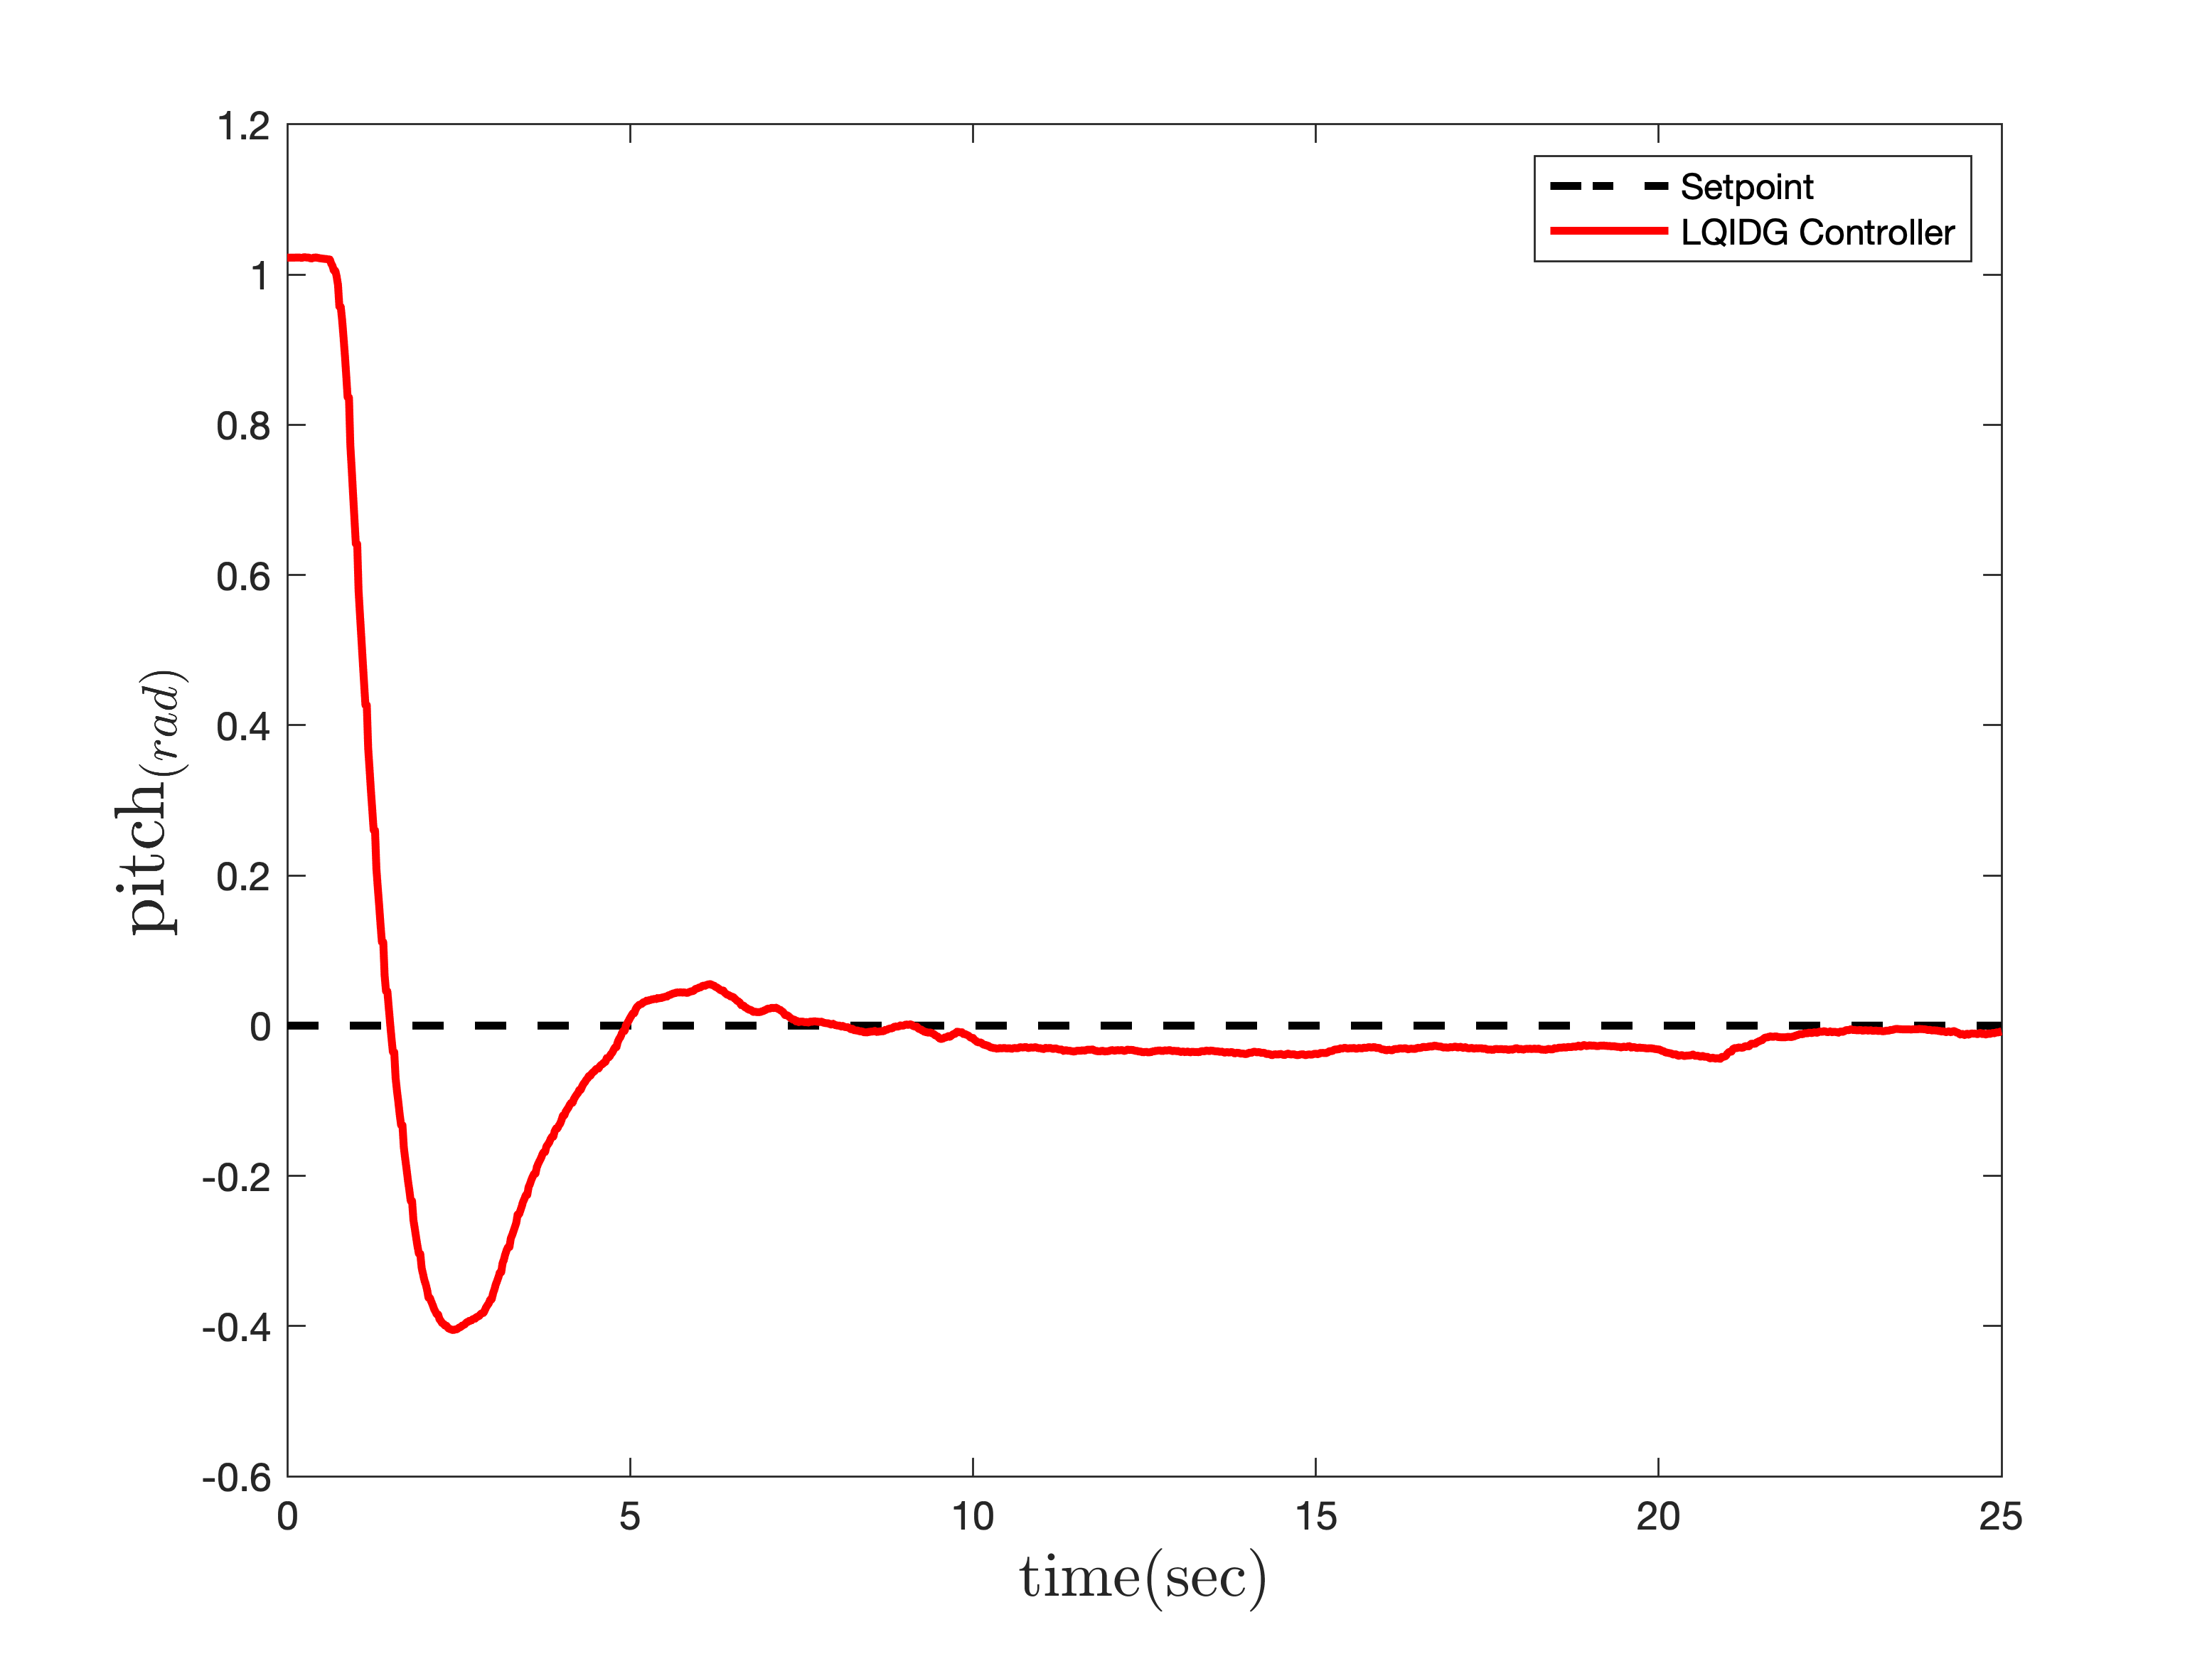
\includegraphics[width=.49\linewidth]{../Figures/Calibration/LQIDG/3DOF/lqidg_pitch.png}\label{fig:pitch}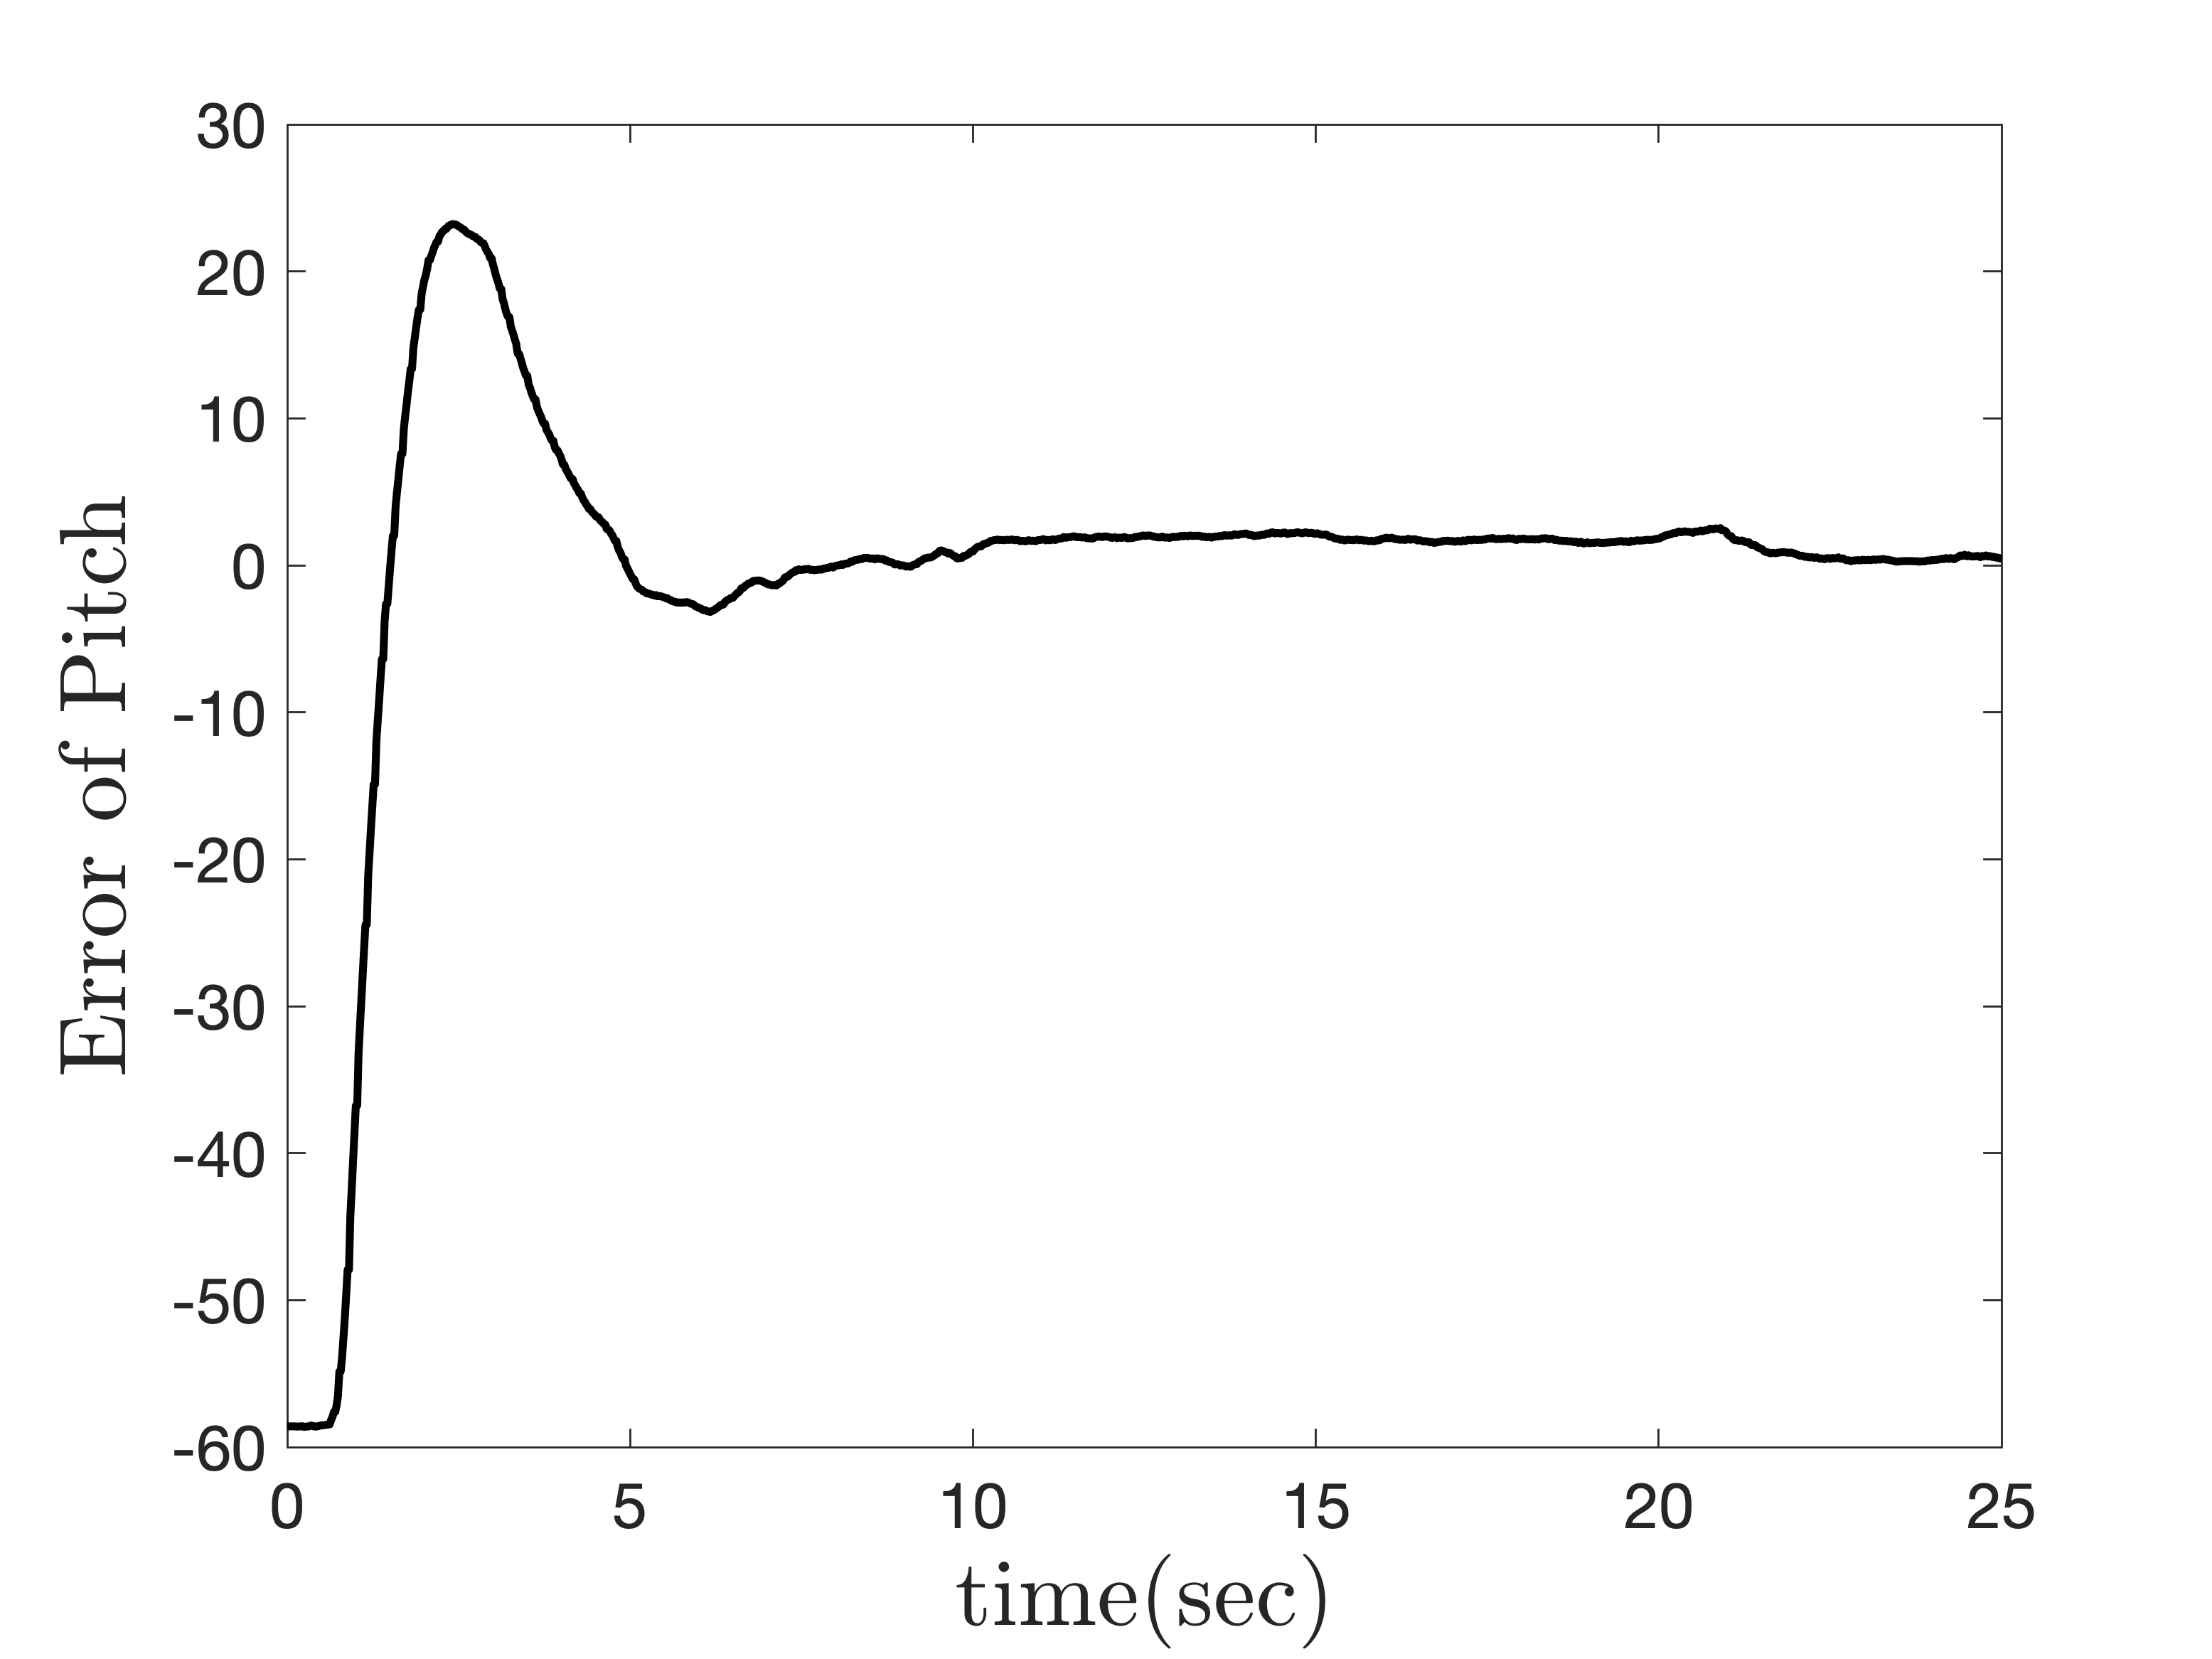
\includegraphics[width=.49\linewidth]{../Figures/Calibration/LQIDG/3DOF/lqidg_pitch_e.png}
	}
	\hfil
	\subfloat[]{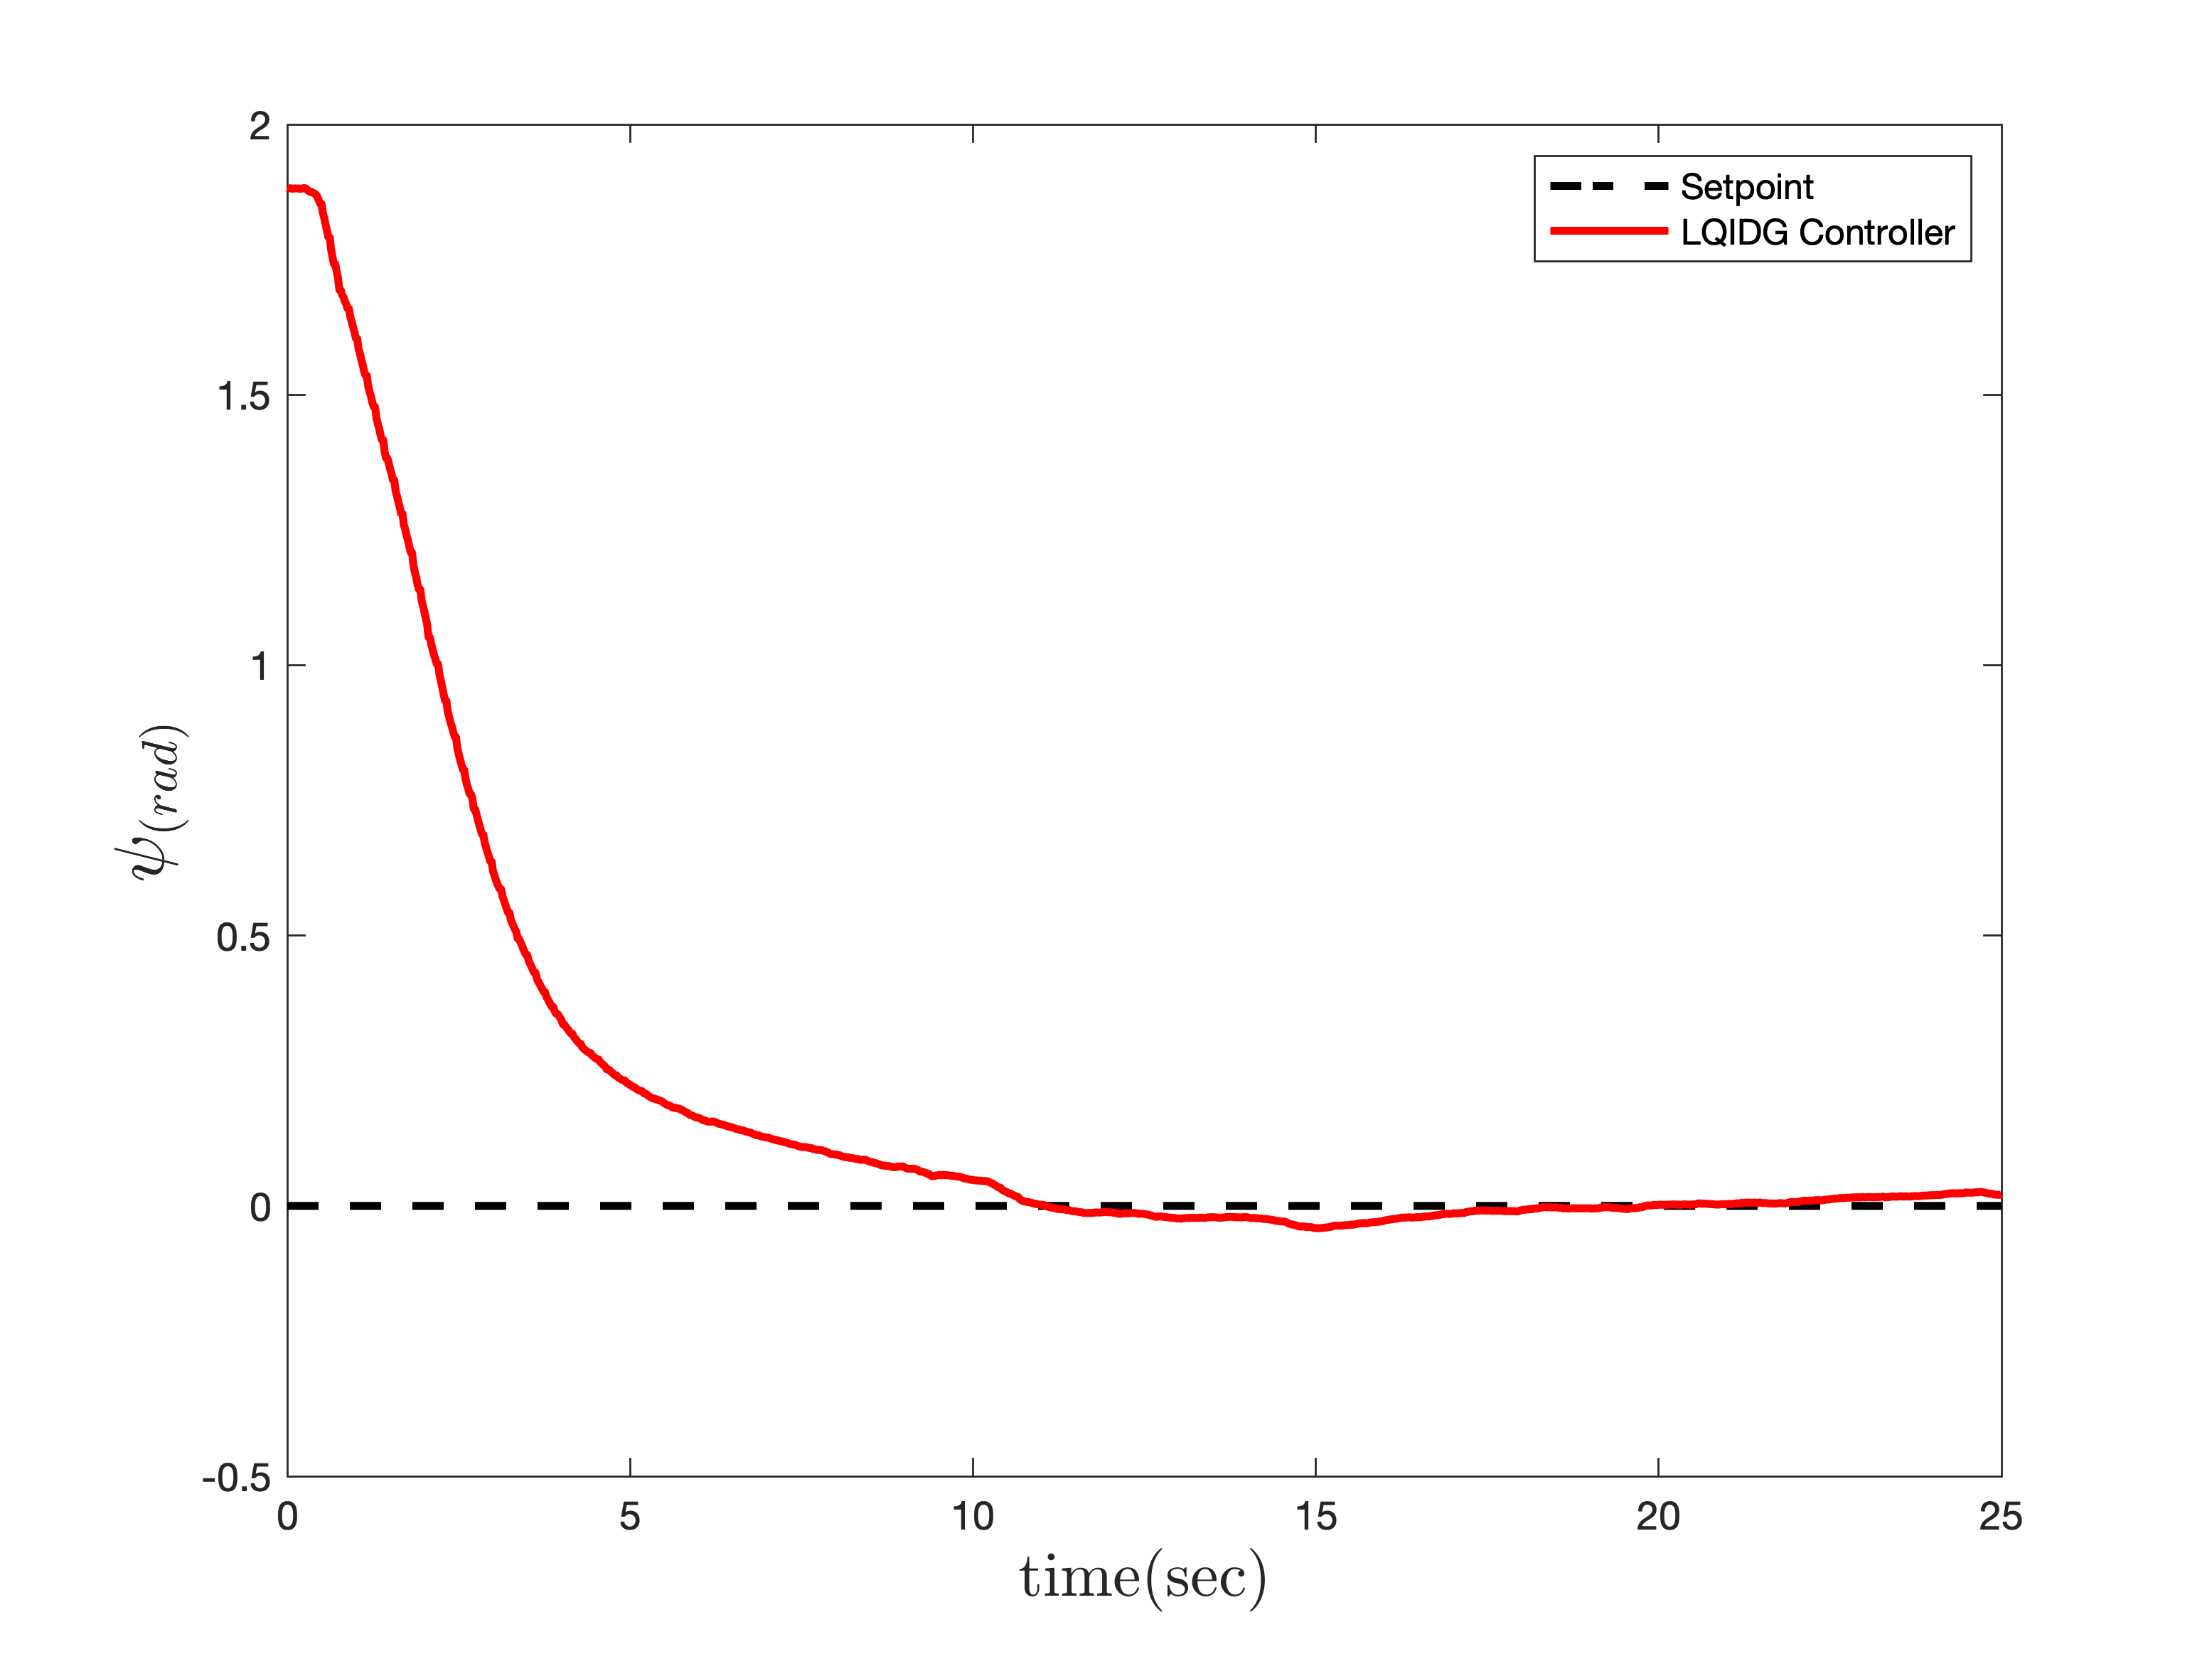
\includegraphics[width=.49\linewidth]{../Figures/Calibration/LQIDG/3DOF/lqidg_yaw.png}\label{fig:yaw}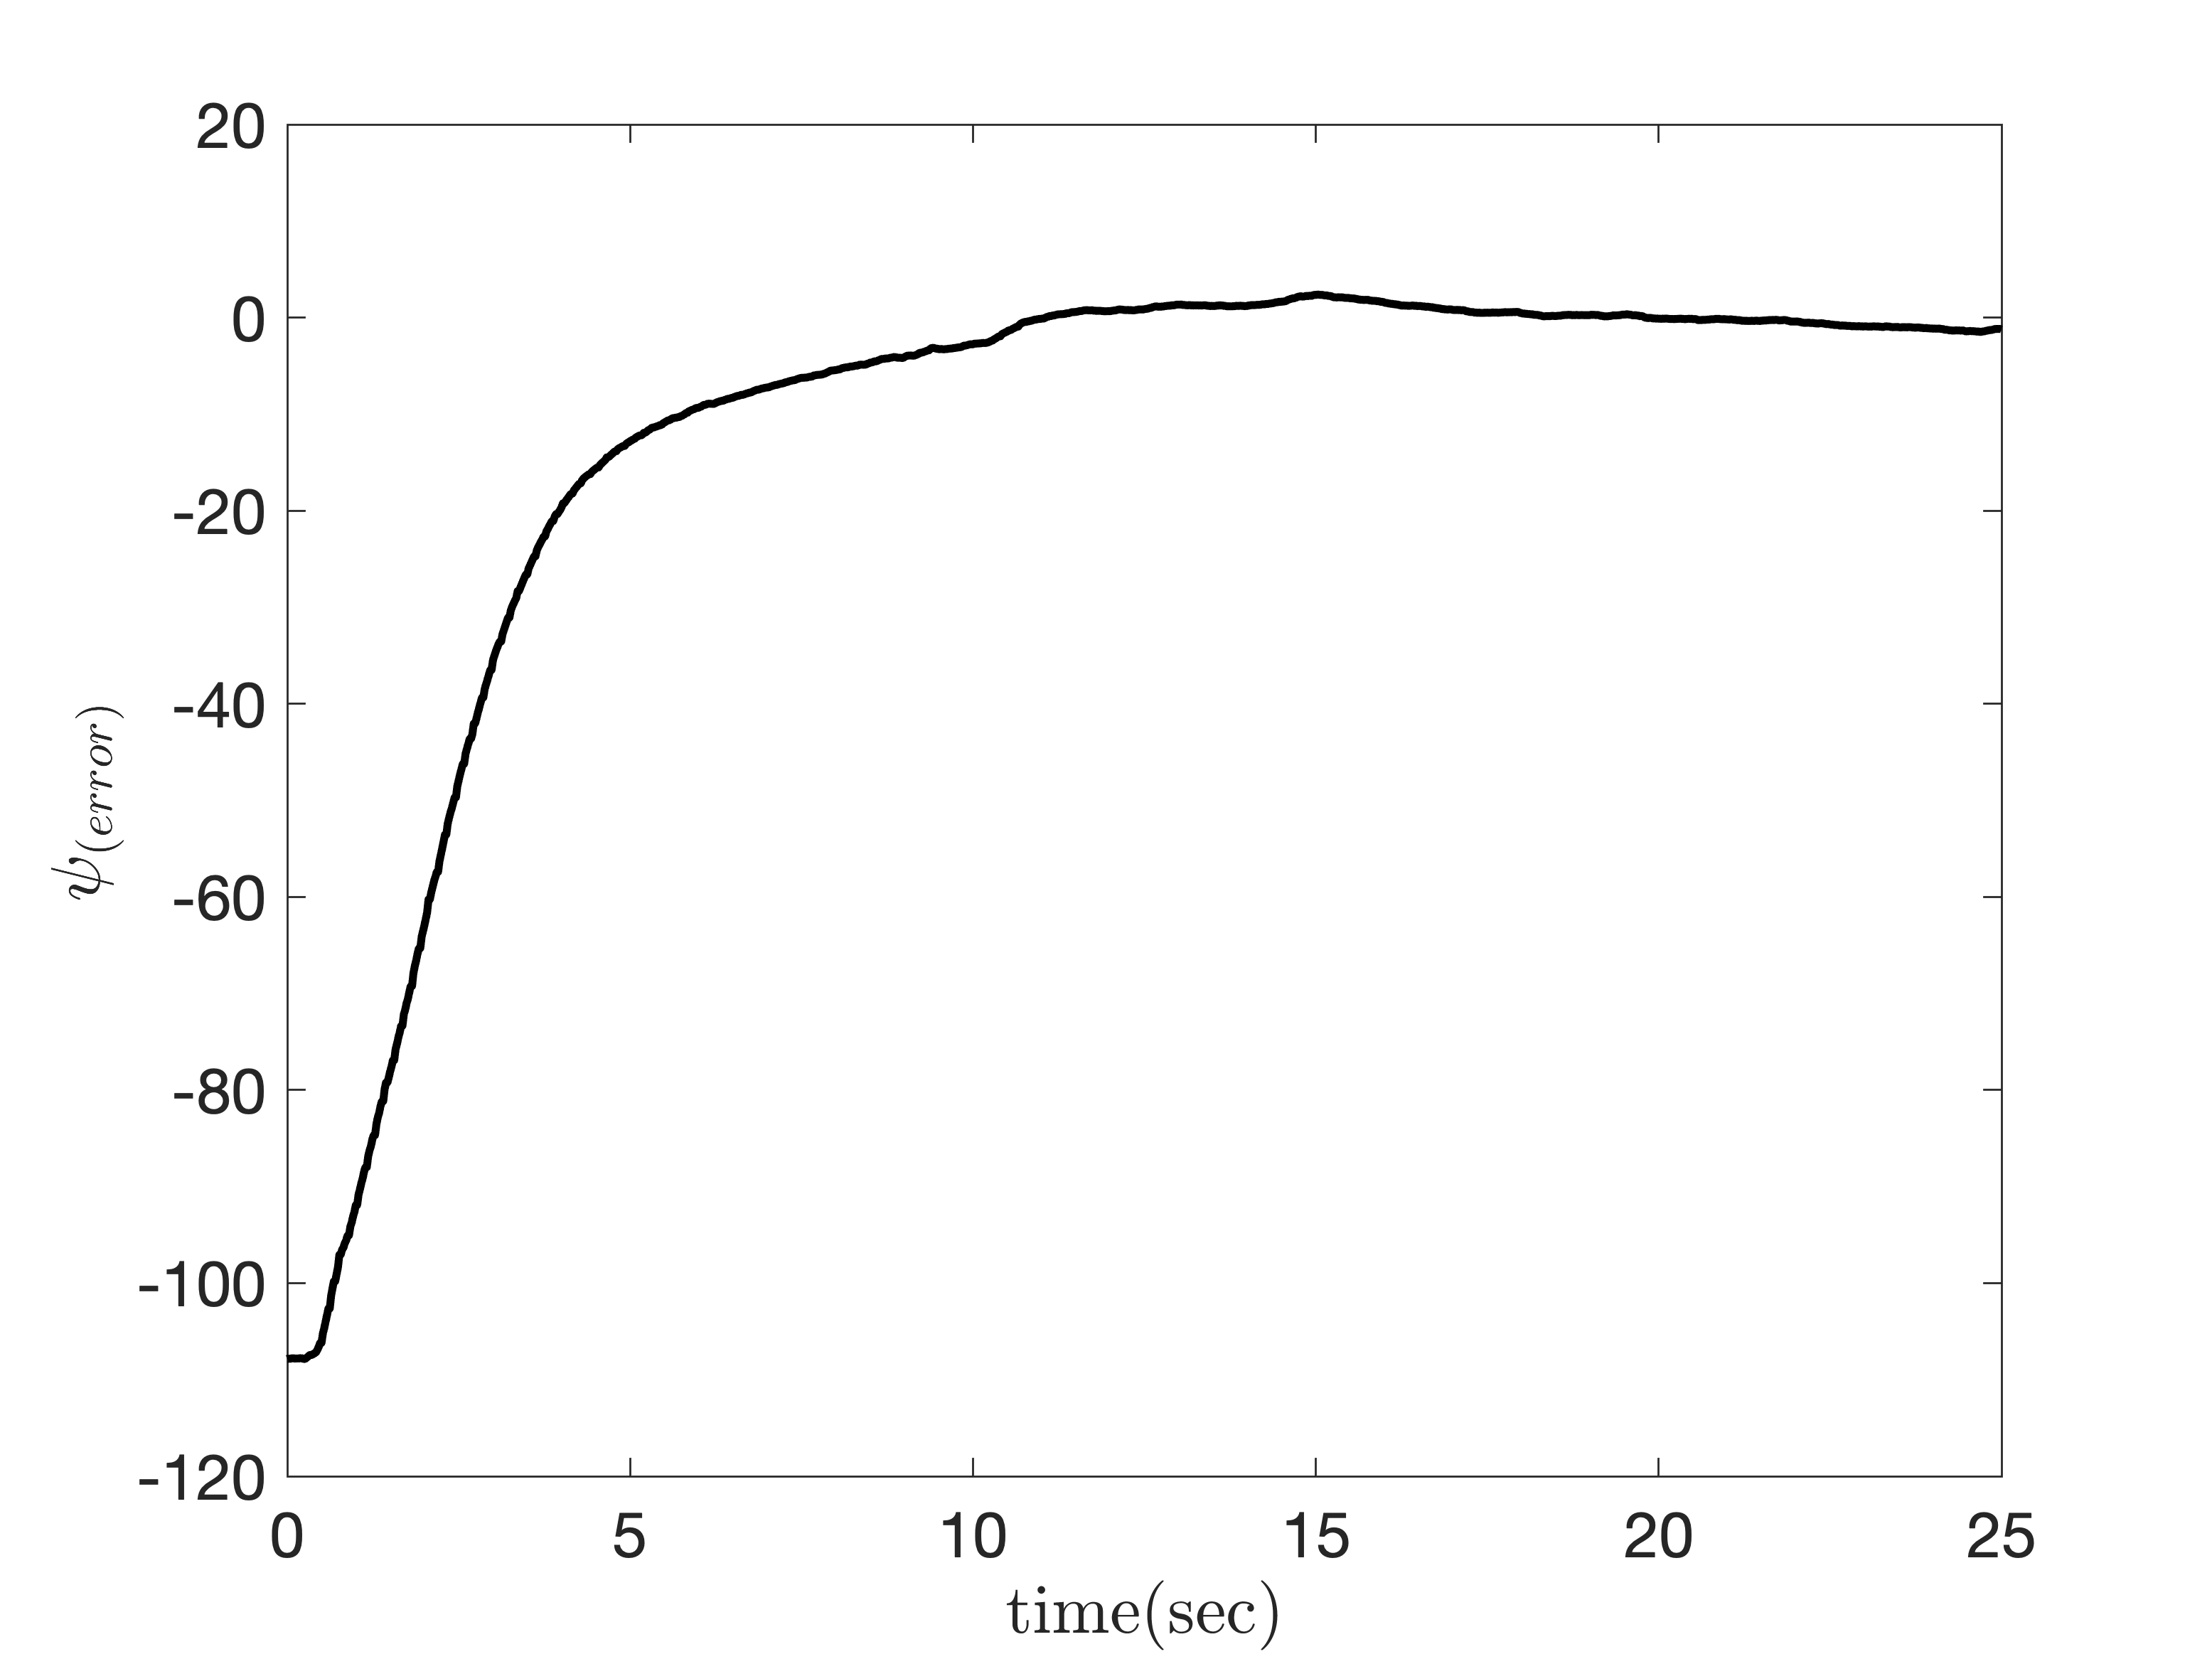
\includegraphics[width=.49\linewidth]{../Figures/Calibration/LQIDG/3DOF/lqidg_yaw_e.png}
	}
	\caption{Performance of the LQIR-GT controller (a) roll angle (b) pitch angle (c) actual yaw}
	\label{fig:result}
\end{figure}

\begin{figure}[!h]
	\centering
	\subfloat{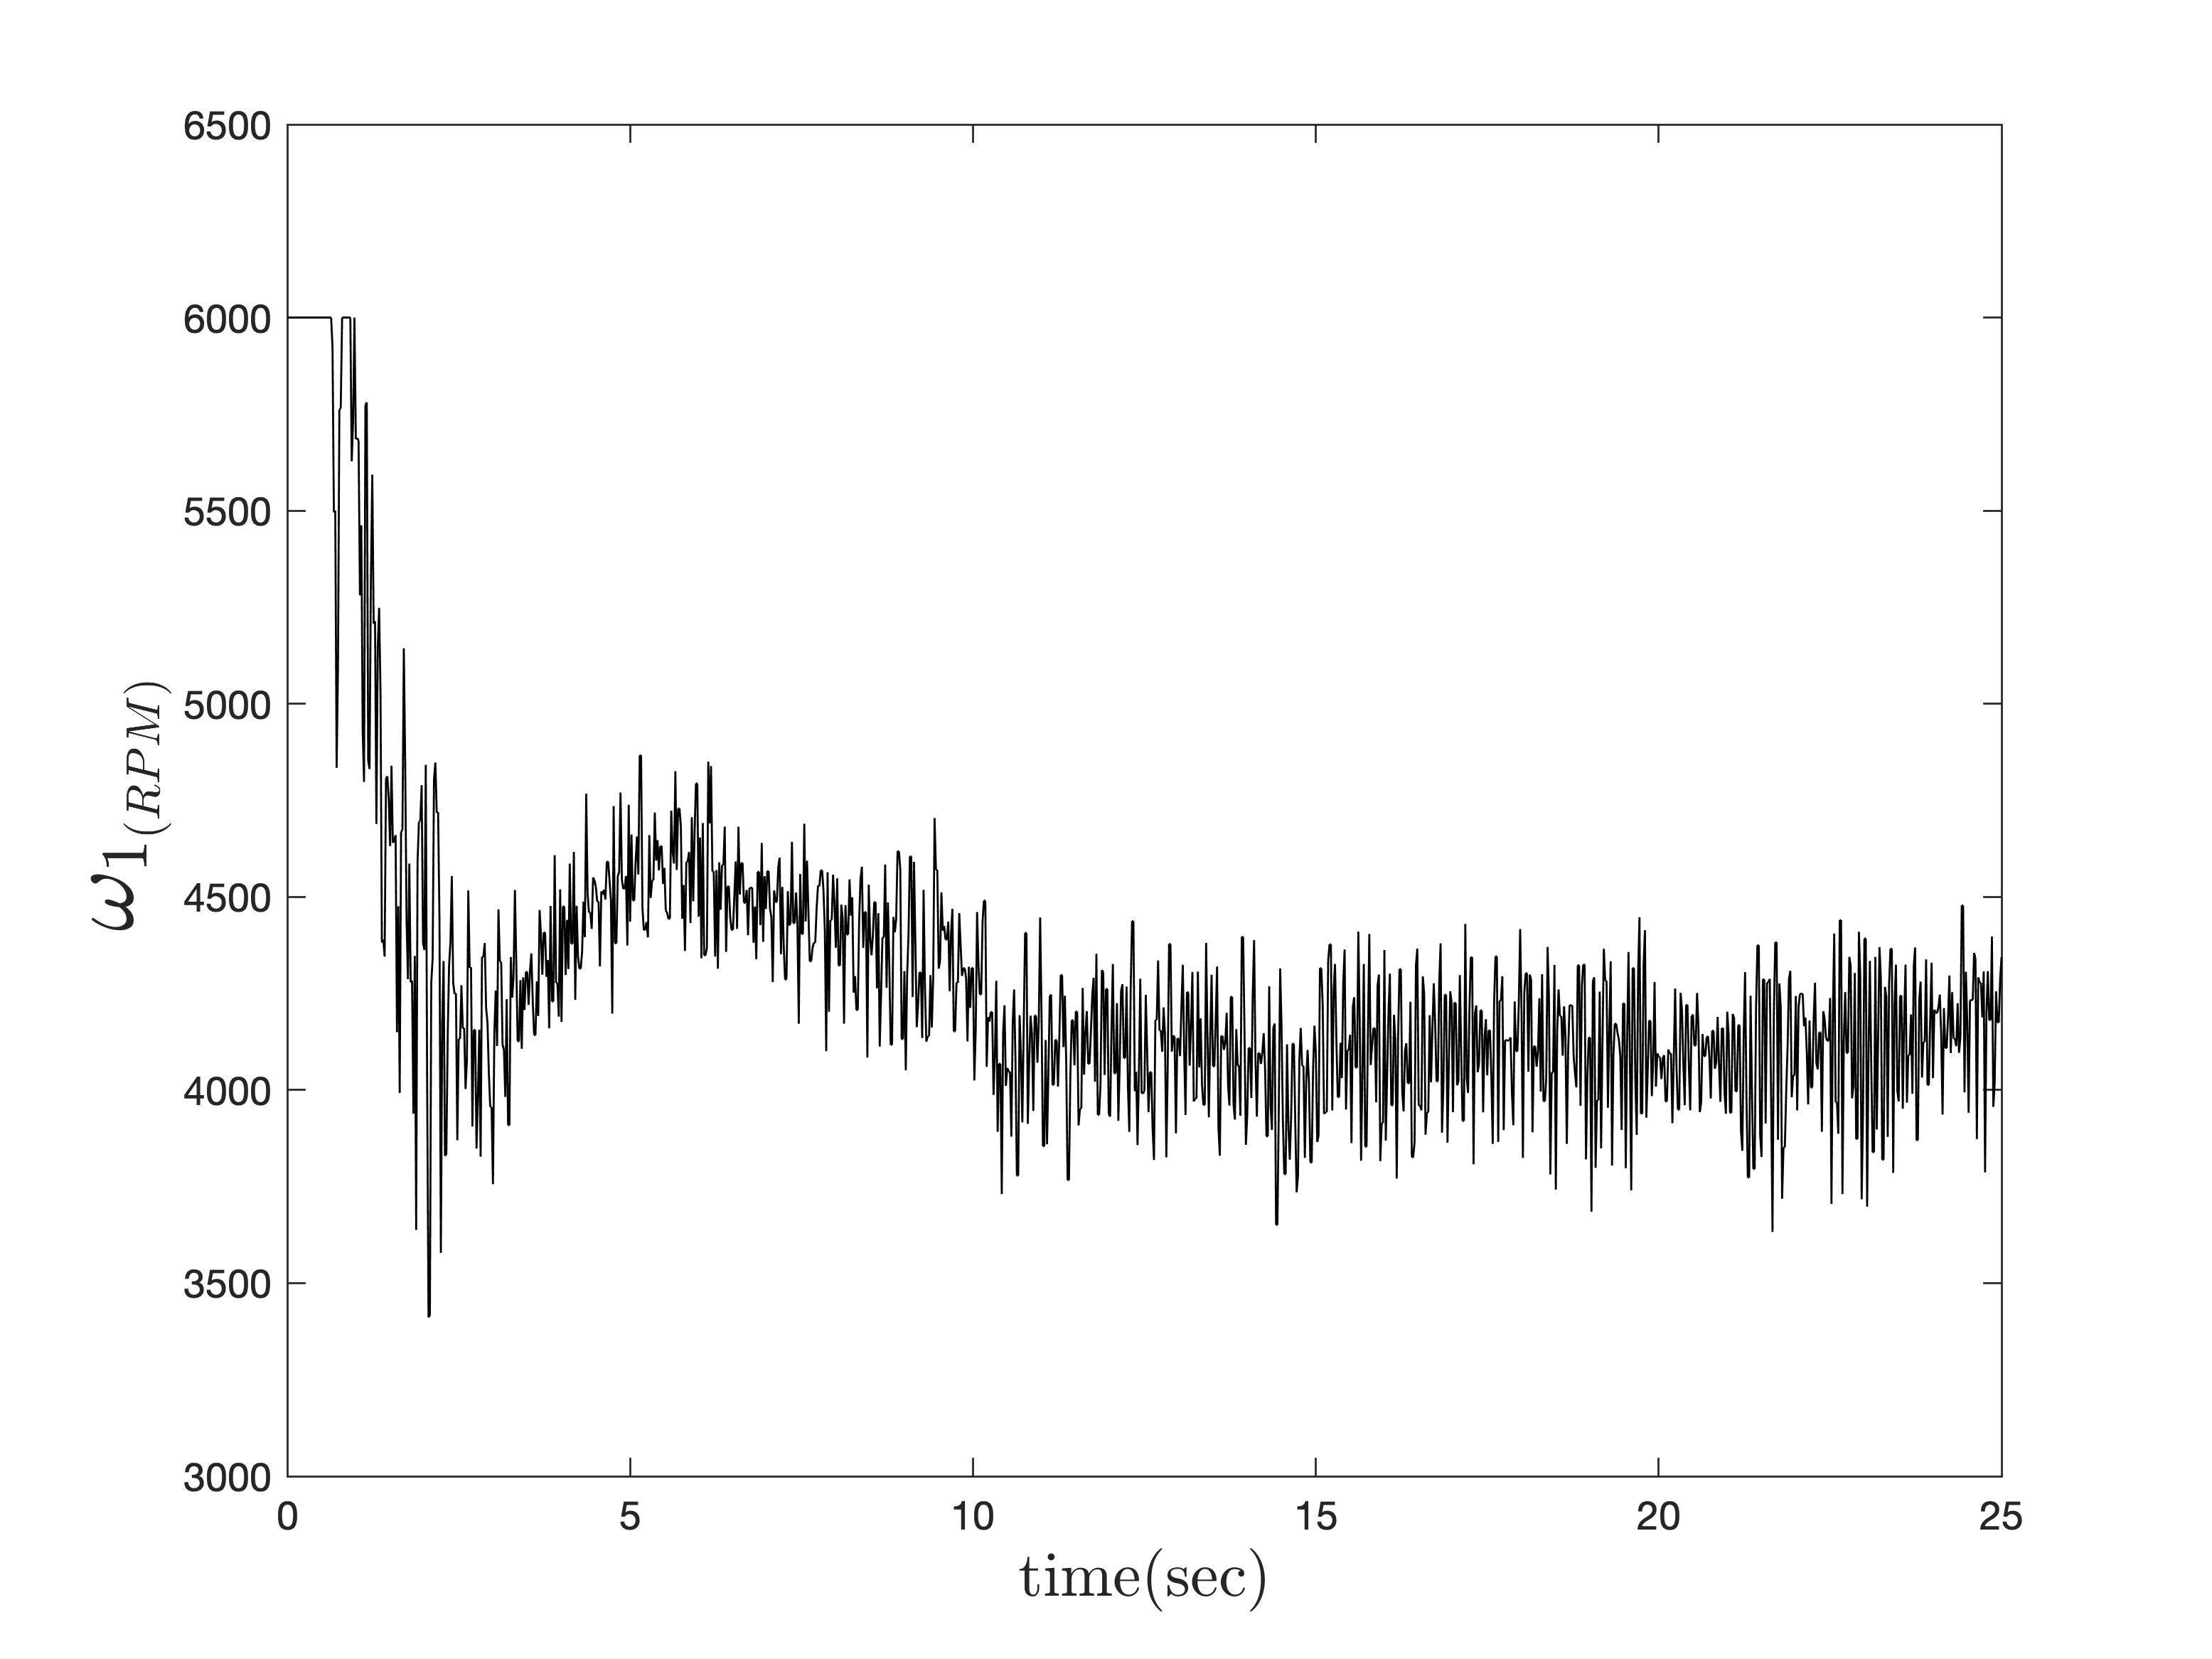
\includegraphics[width=.49\linewidth]{../Figures/Calibration/LQIDG/3DOF/lqidg_Omega_1.png}
	}
	\subfloat{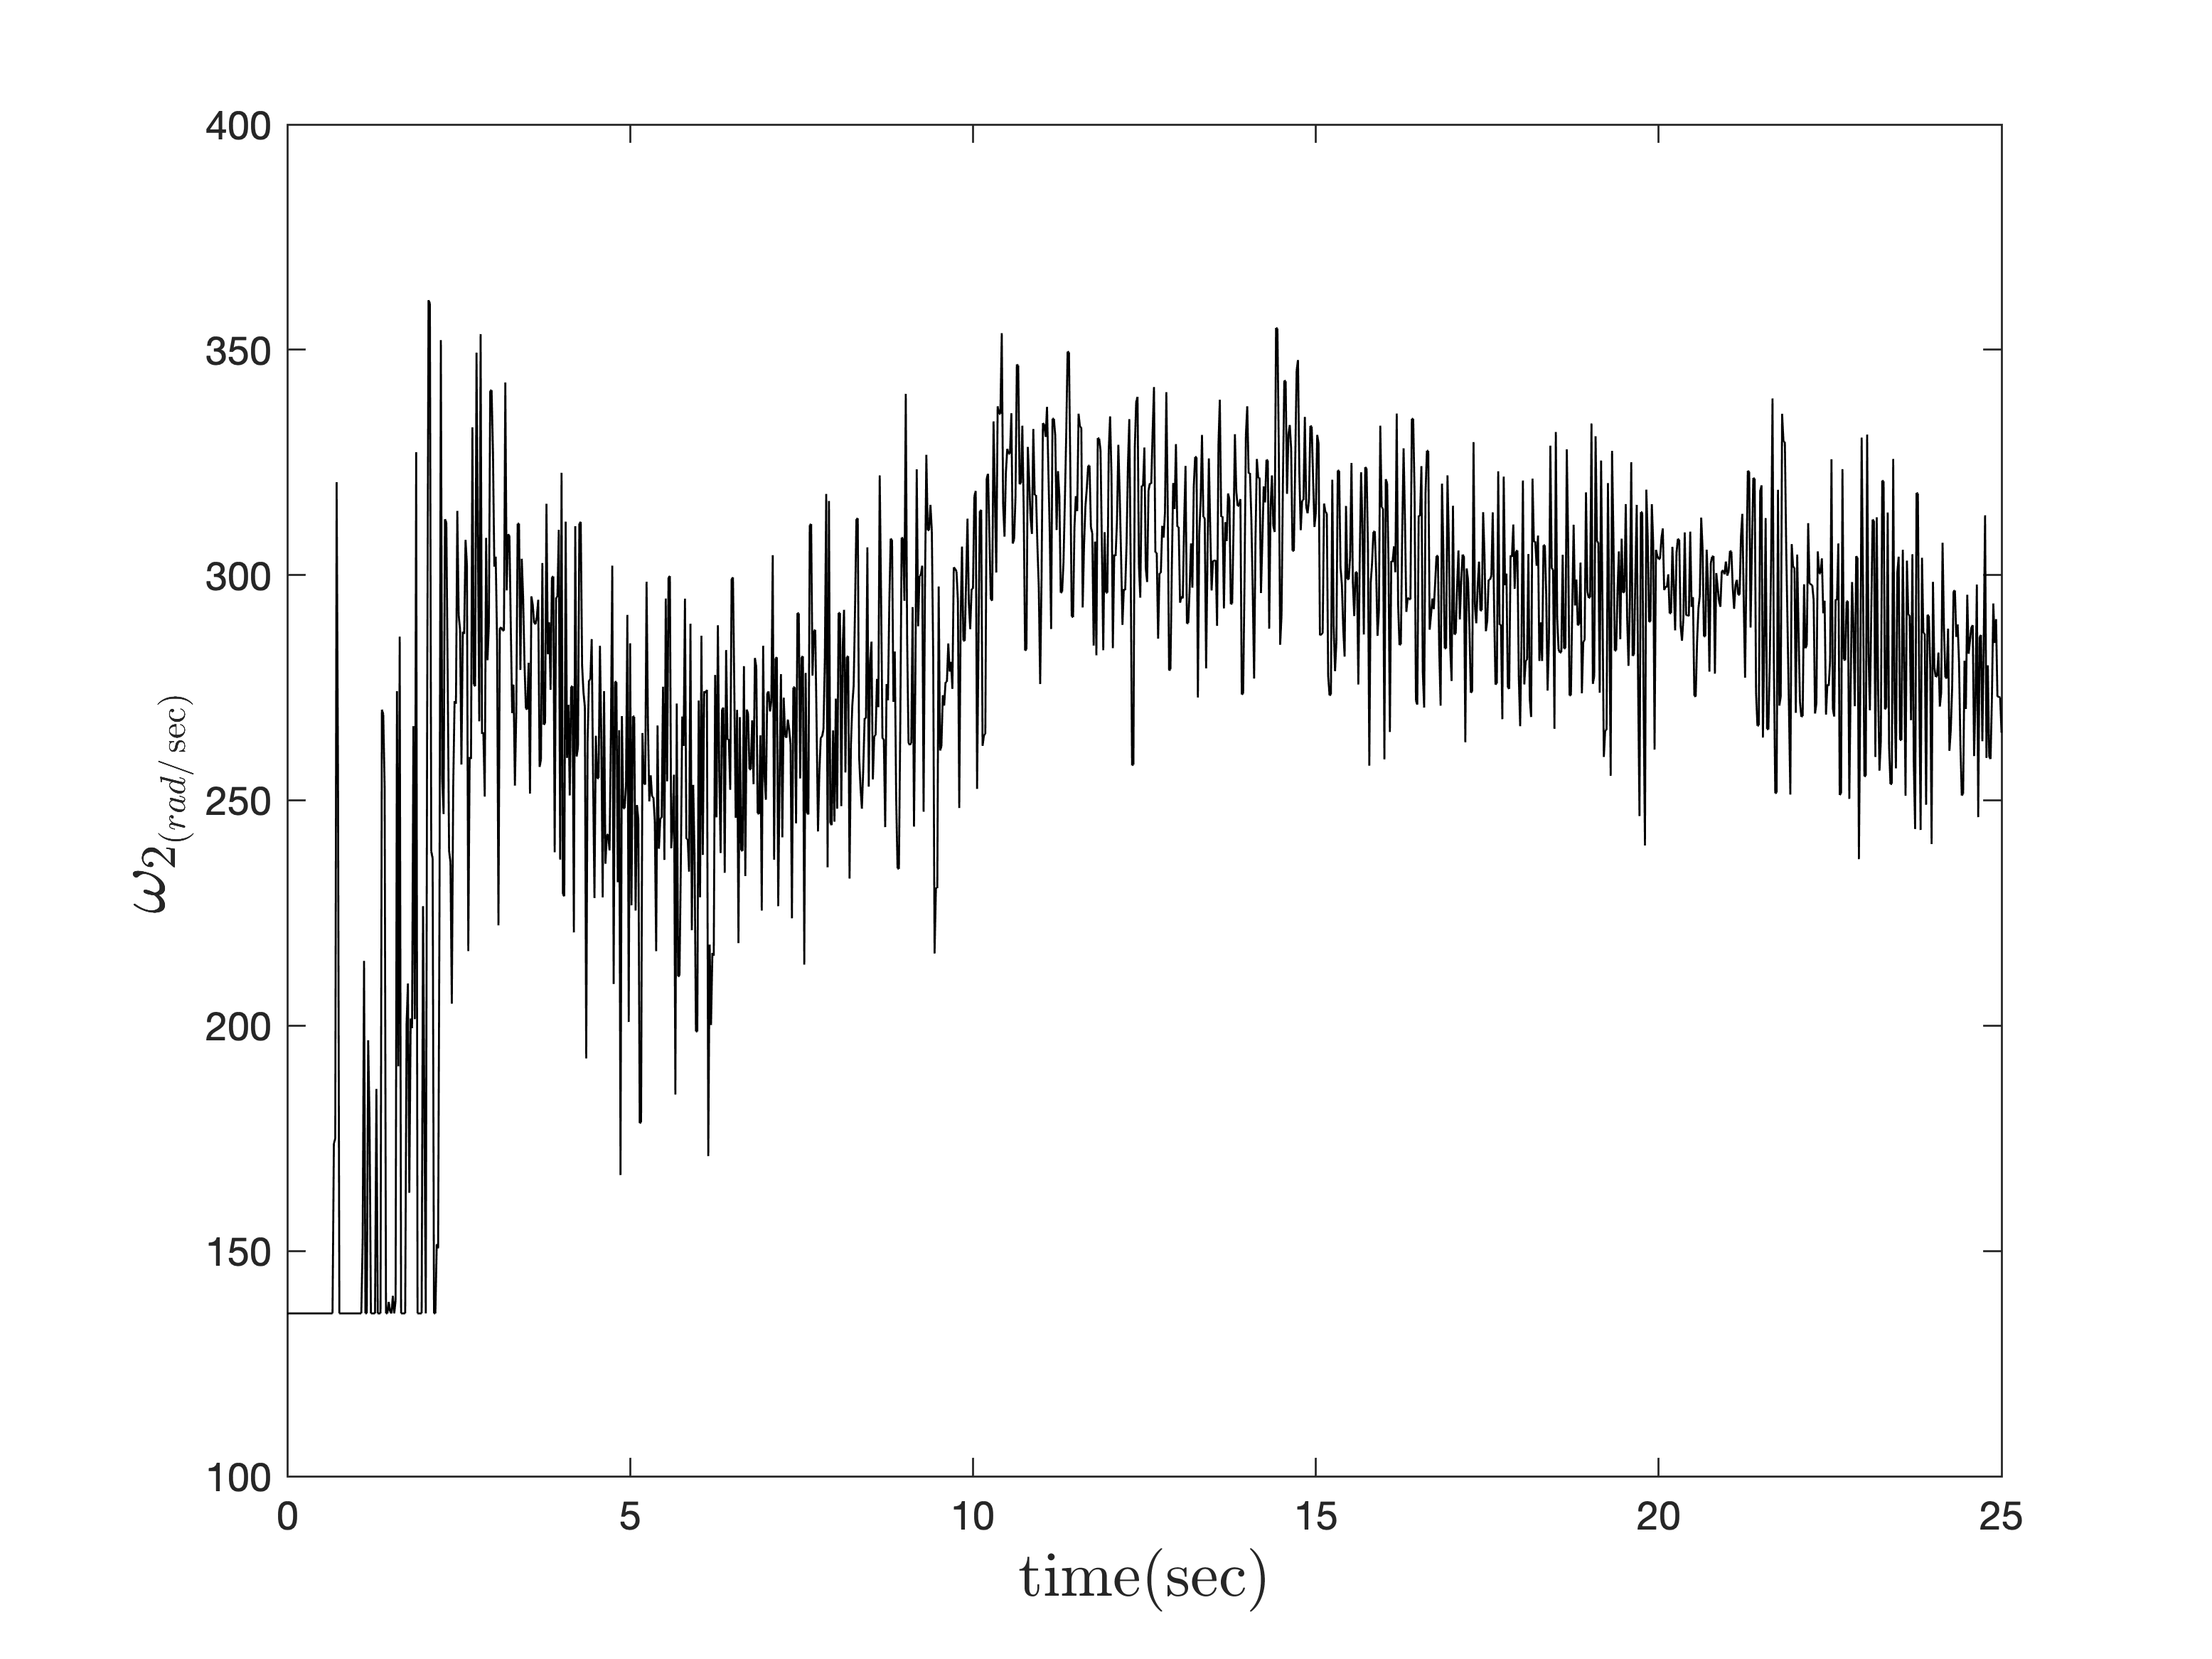
\includegraphics[width=.49\linewidth]{../Figures/Calibration/LQIDG/3DOF/lqidg_Omega_2.png}
	}
	\hfil
	\subfloat{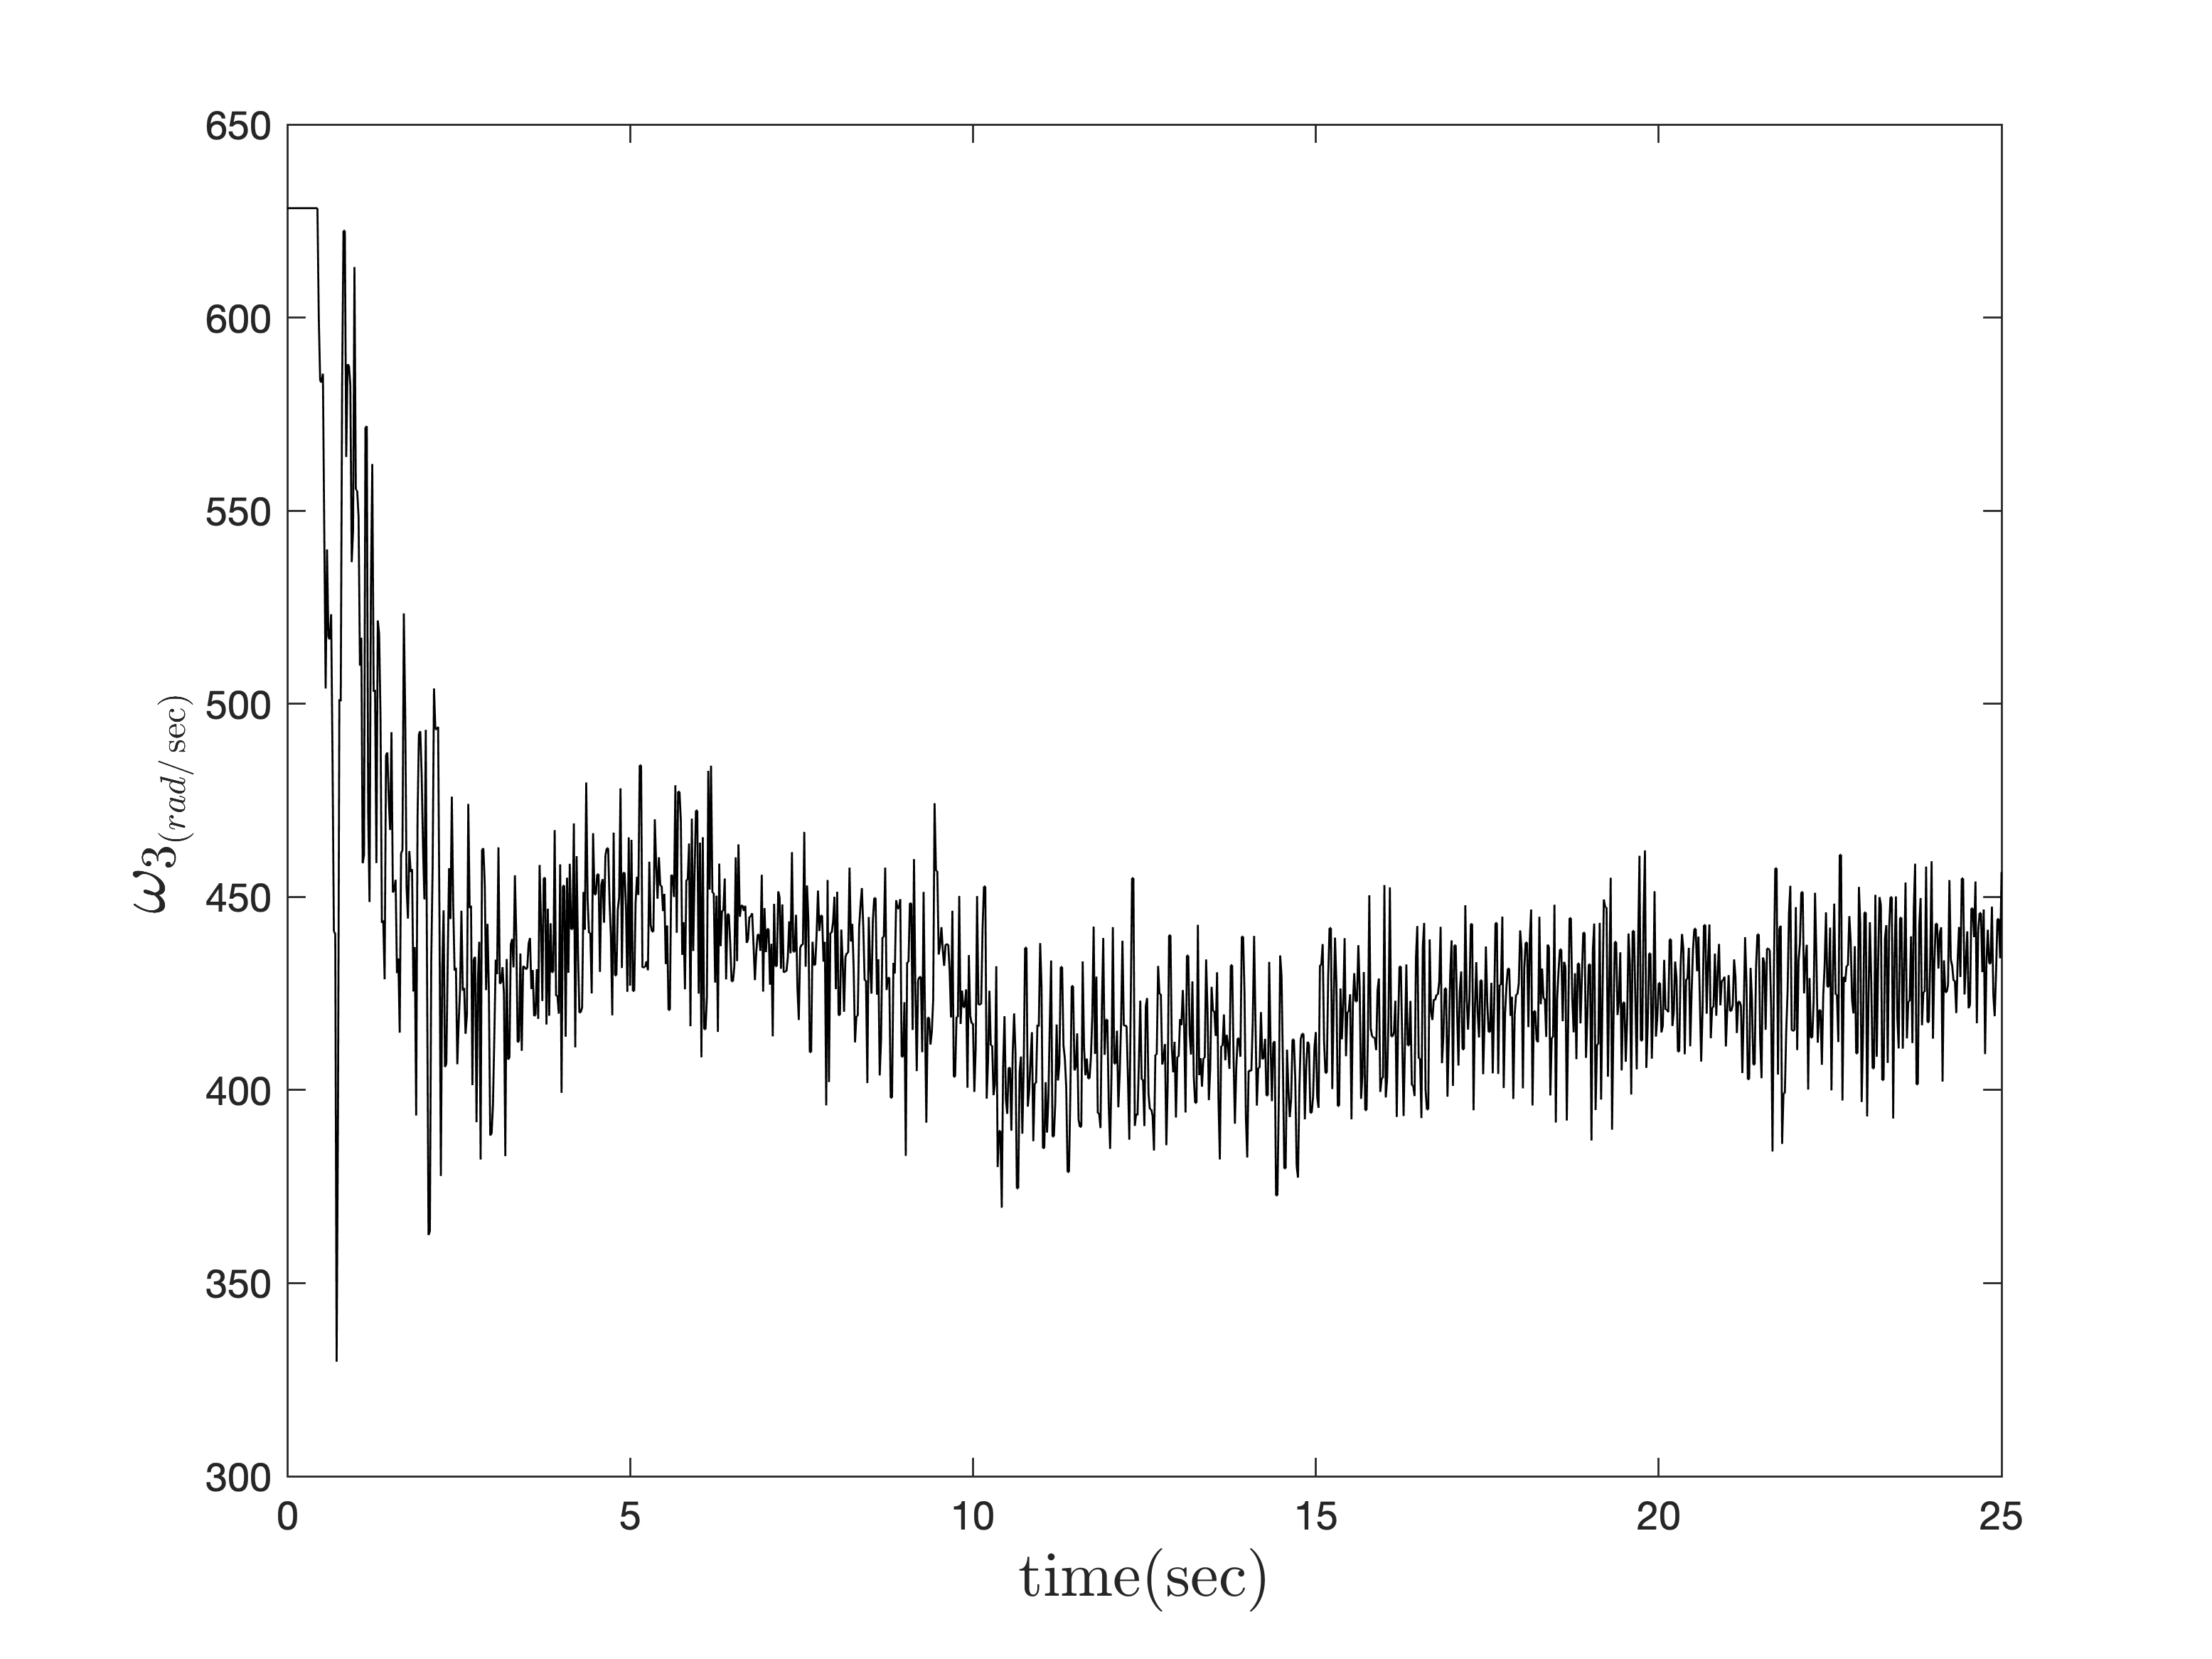
\includegraphics[width=.49\linewidth]{../Figures/Calibration/LQIDG/3DOF/lqidg_Omega_3.png}
	}
	\subfloat{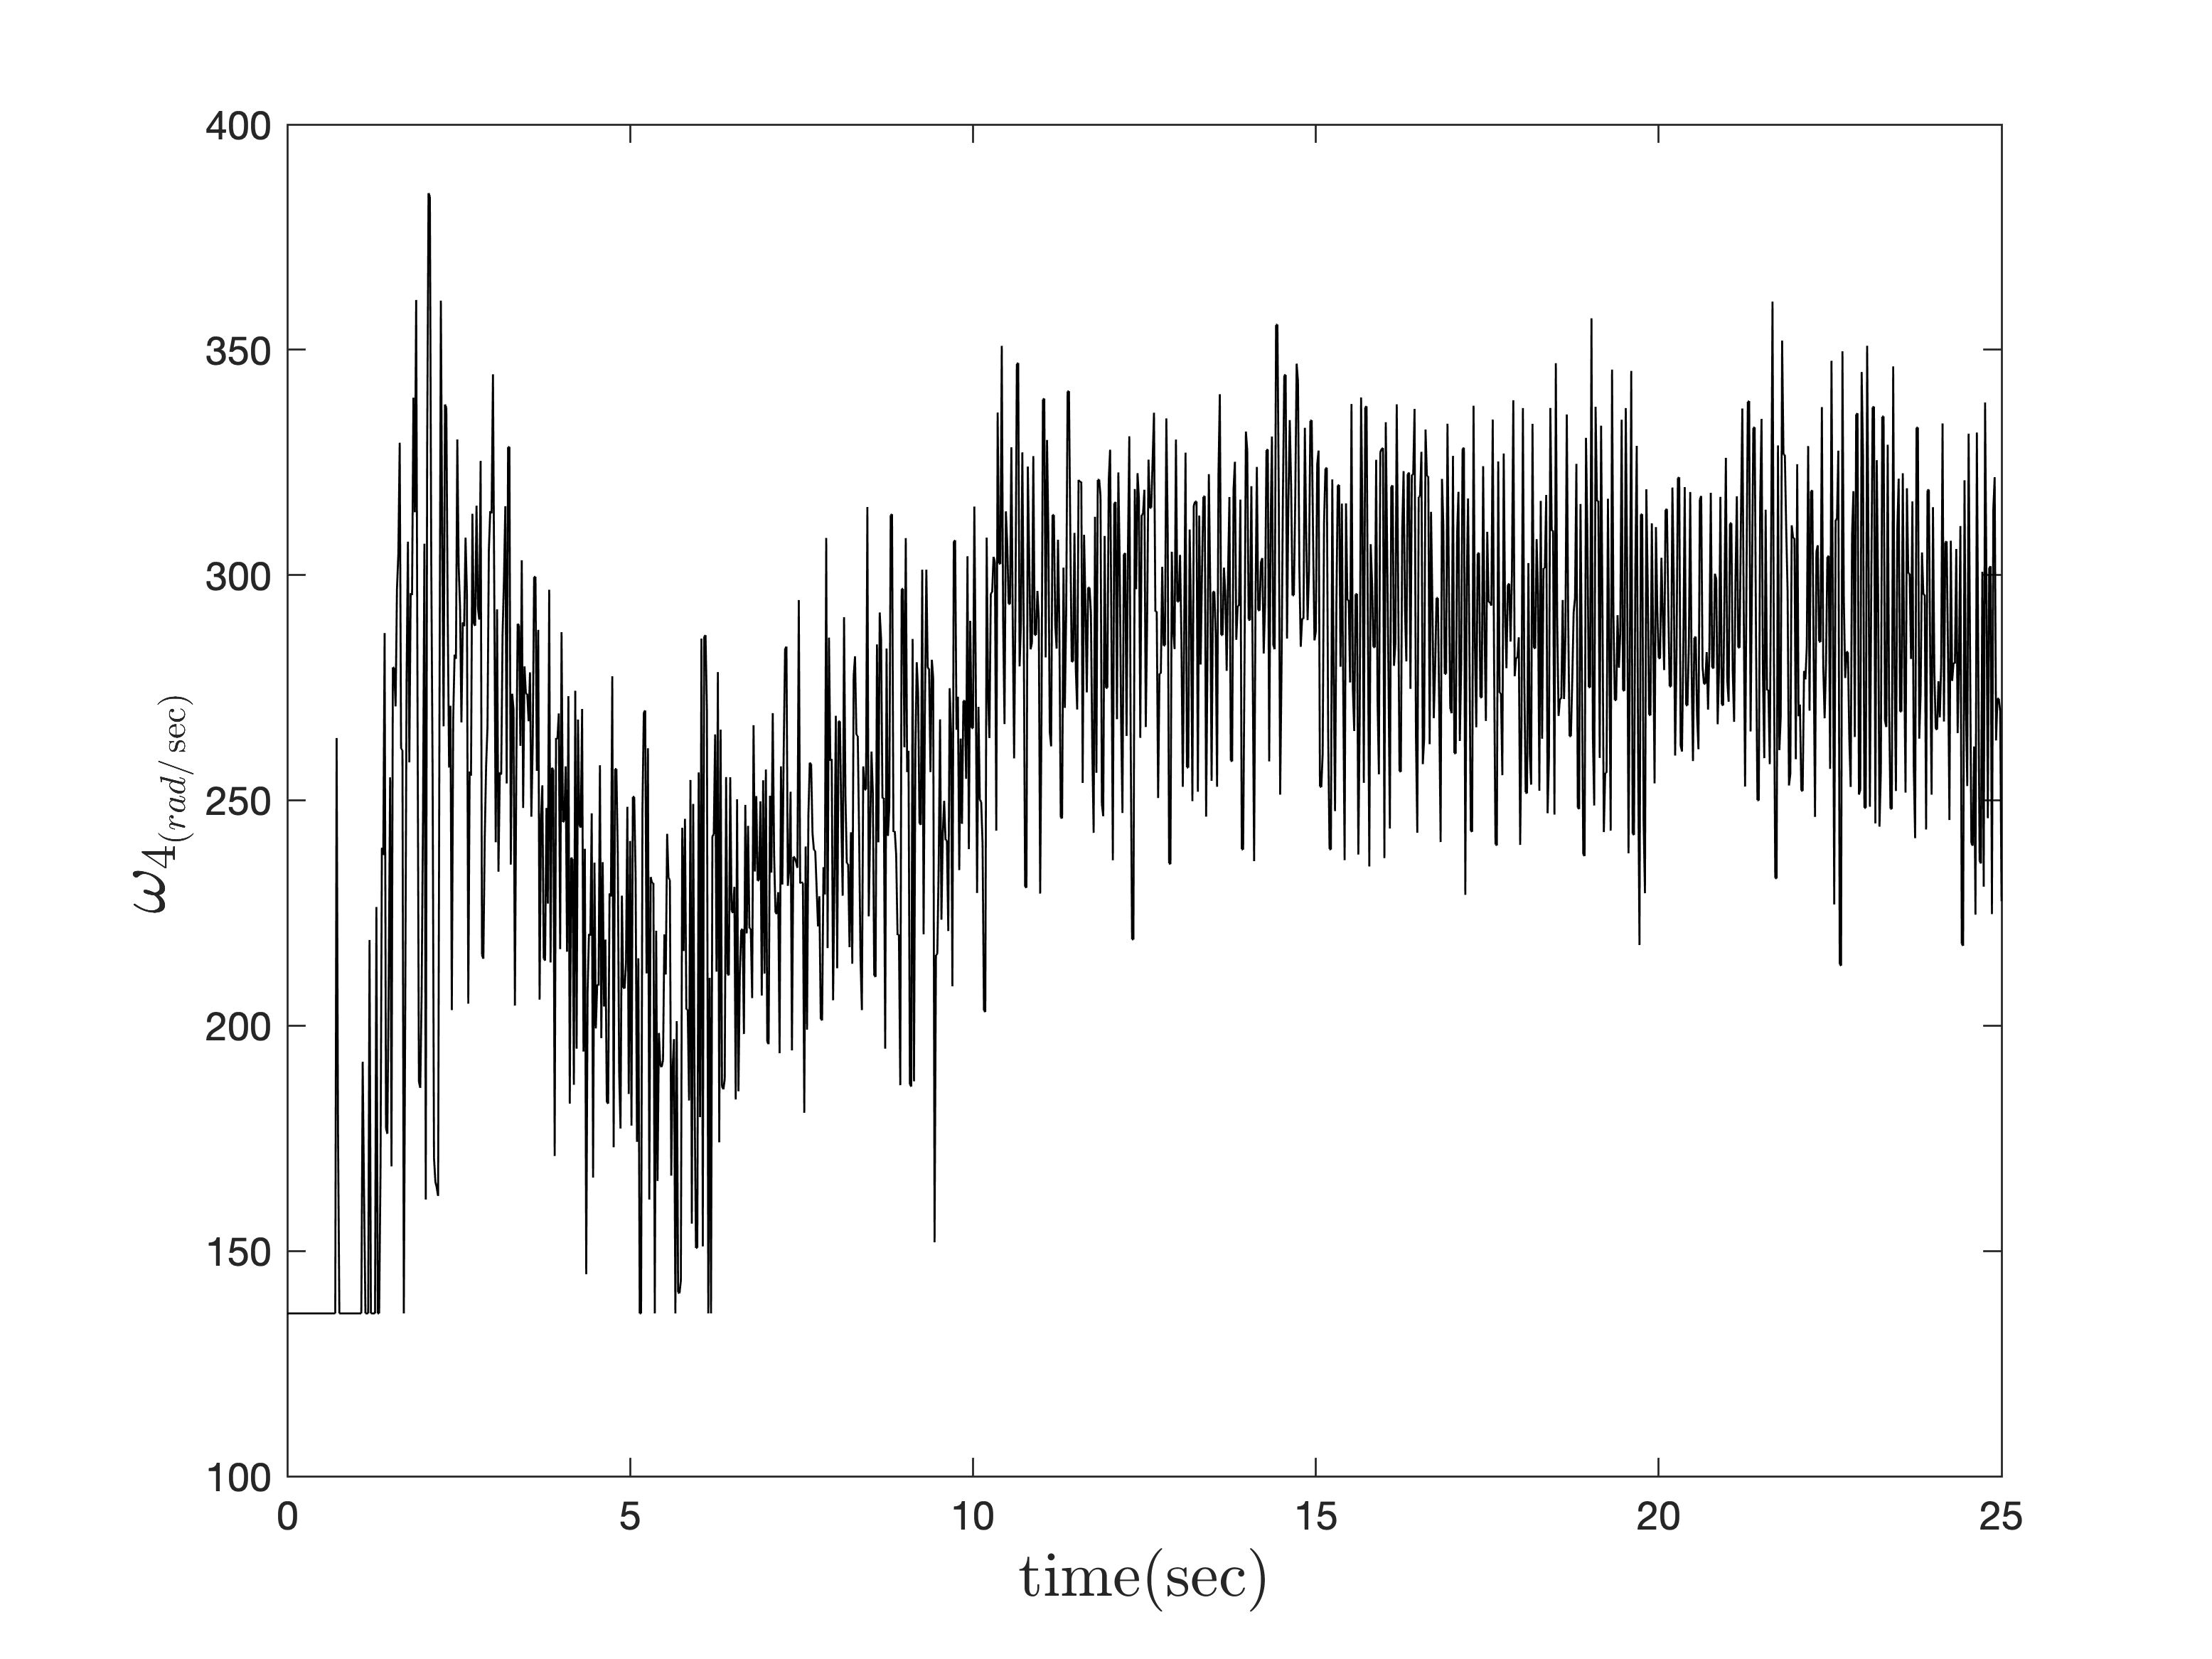
\includegraphics[width=.49\linewidth]{../Figures/Calibration/LQIDG/3DOF/lqidg_Omega_4.png}
	}
	\caption{Time history of angular velocity commands}
	\label{fig:omega}
\end{figure}



\subsection{Comparison with LQR}
\noindent Here, the LQIR-DG controller performance is compared with famous control strategy such as LQR controller method. \figurename{\ref{fig:compare}} compares the quadrotor's desired and actual pitch angle in the presence of these controllers. This results indicates that the LQIR-DG controller can provide high tracking performance, such as good transient response and high rapid convergence relative to LQR controller for pitch angle control of the experimental setup of the quadrotor.
\begin{figure}[!h]
	\centering
	{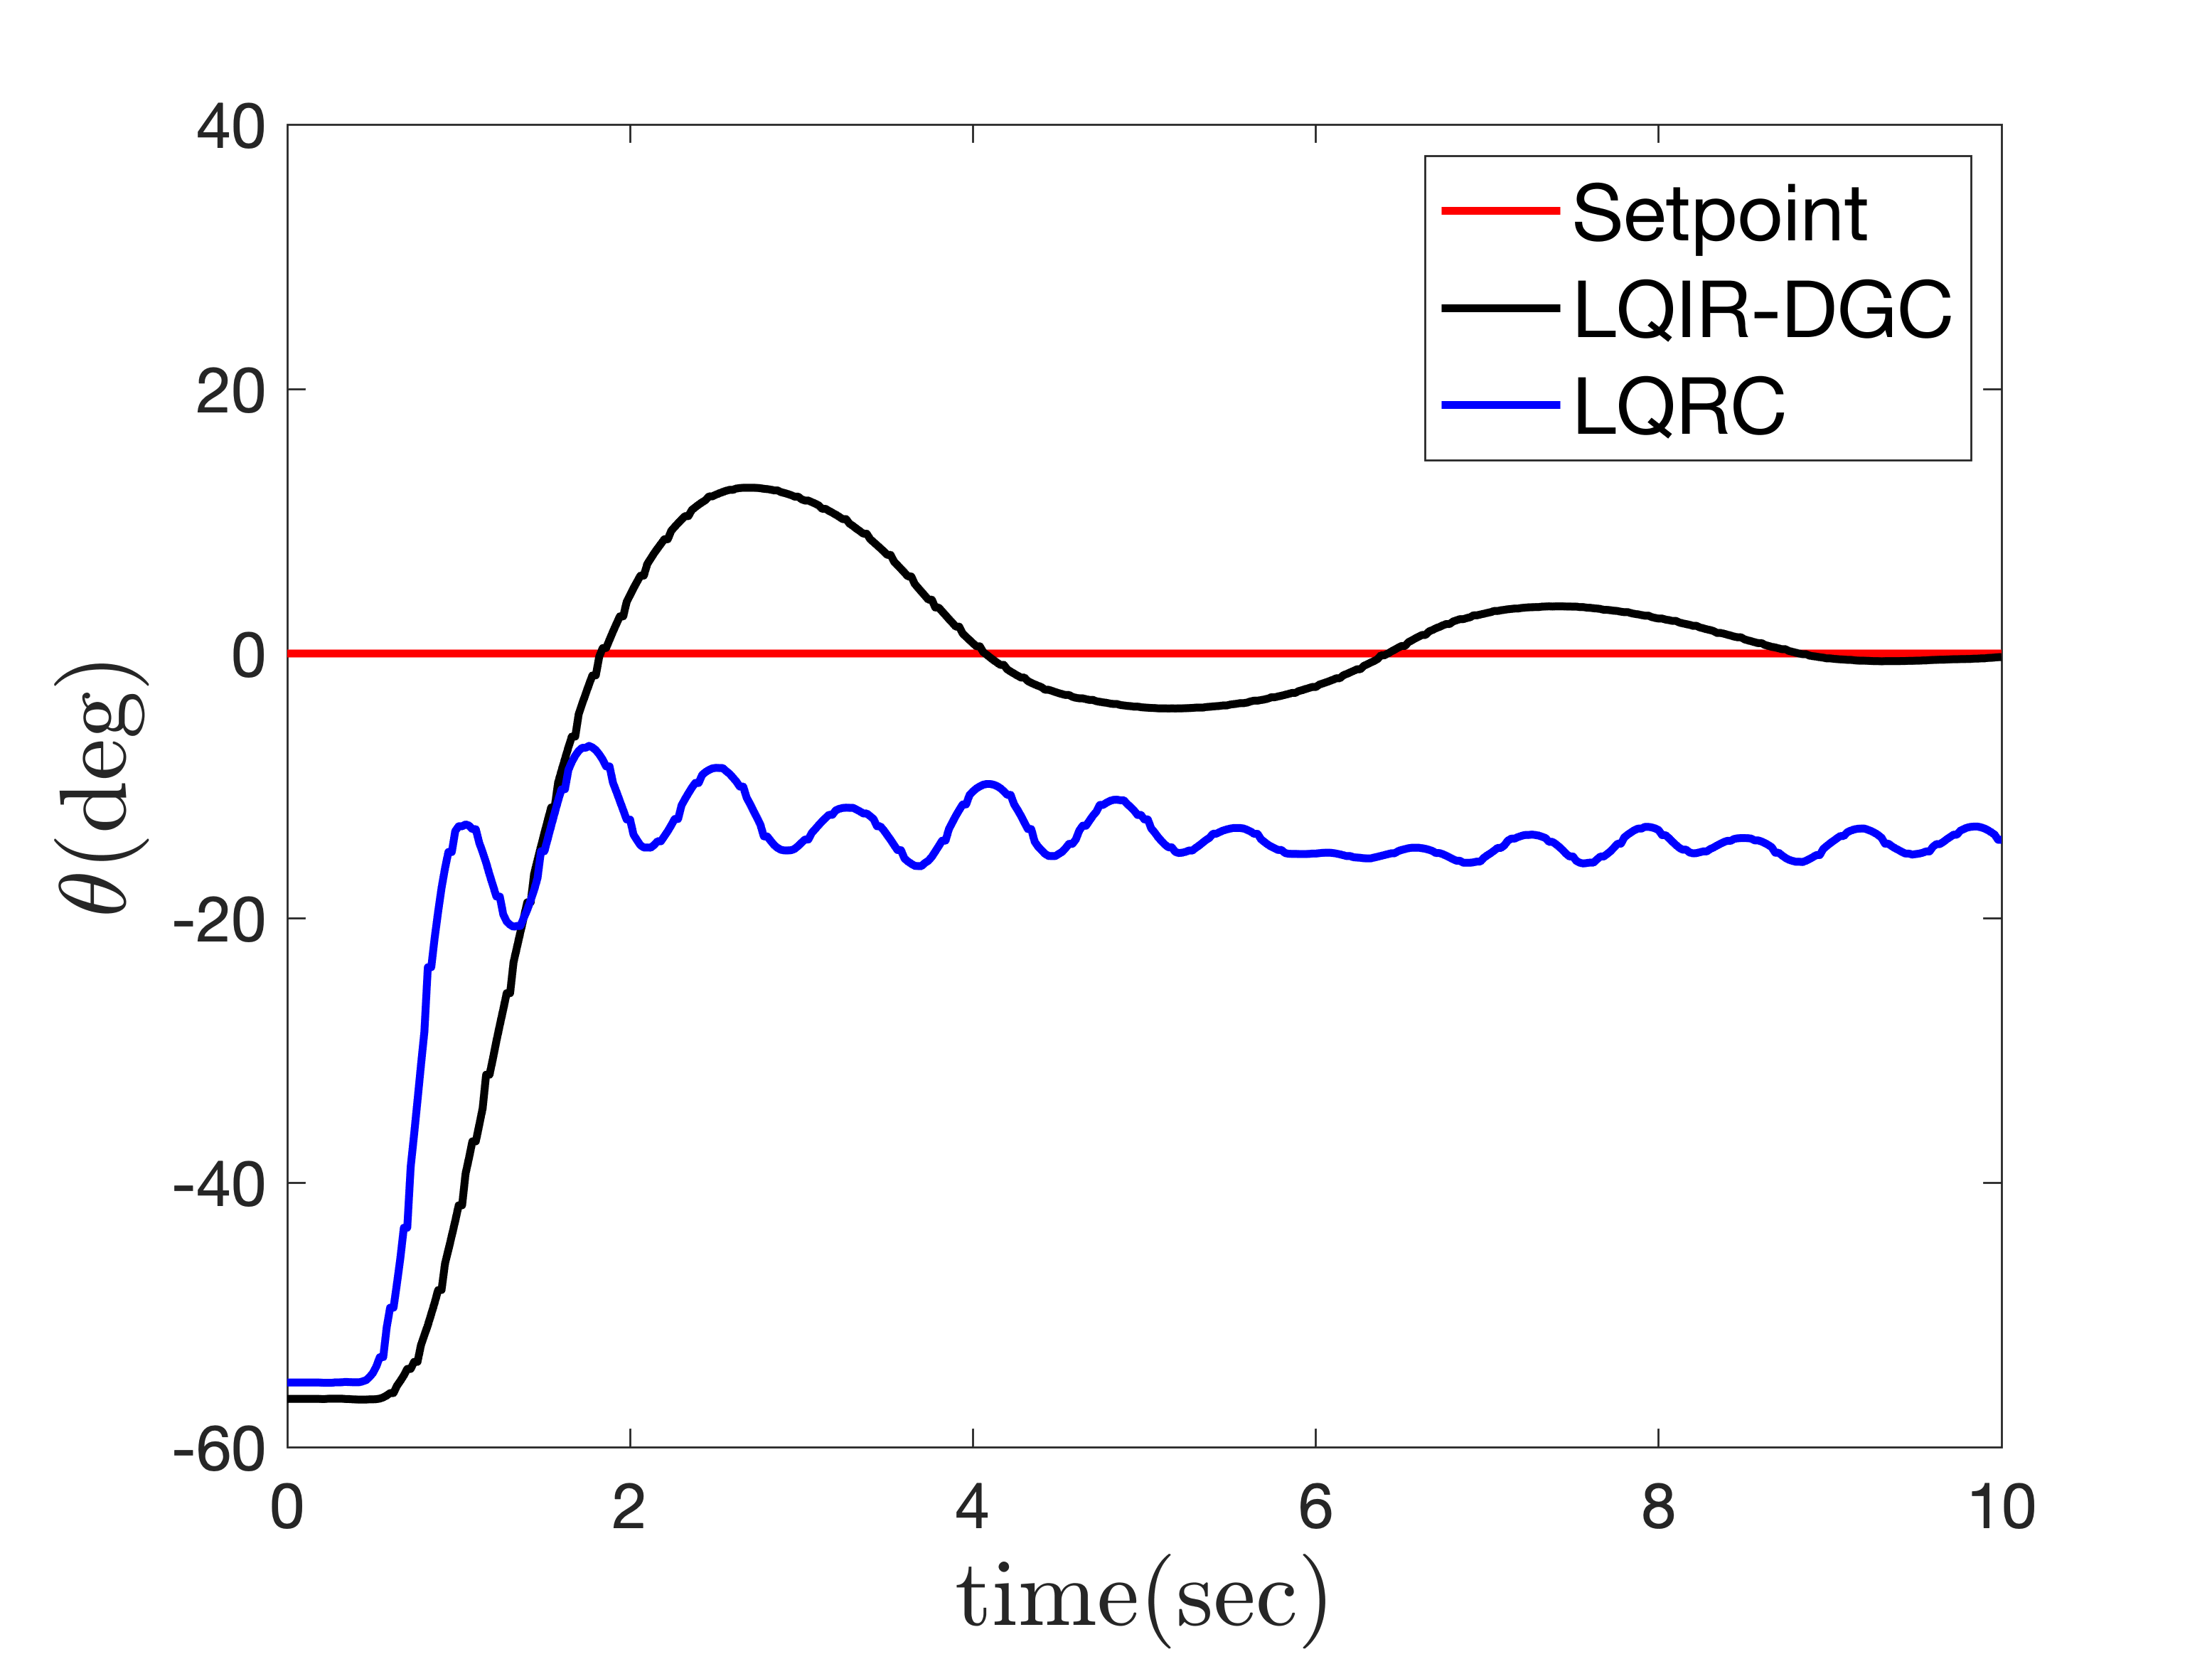
\includegraphics[width=.9\linewidth]{../Figures/Calibration/LQIDGvsLQR/Pitch/lqidgvslqr_pitch.png}
	}
	\caption{Comparison of the LQIR-DG to the LQR in control of the pitch angle of the experimental setup}
	\label{fig:compare}
\end{figure}
\section{Conclusion}\label{sec:conclusion}
\noindent In this study, a linear quadratic with integral action based on the differential game theory, called LQIR-DG, was implemented for level attitude control in an experimental setup of a quadrotor. To implement the proposed controller structure, first, an accurate dynamic model of the quadrotor was linearized in the state-space form, and then the model parameters were estimated. Next, two players were considered for each of the quadrotor's roll, pitch, and yaw channels. The first player found the best control command for each channel of the setup of a quadrotor based on the mini-maximization of a quadratic criterion; when the second player produced the worst disturbances. Finally, the performance of the proposed controller was evaluated in level flight and compared to the LQR controller. The implementation results verify the successful performance of the LQIR-DG method in the level flight of the attitude control for the actual plant.





\begin{thebibliography}{00}
\bibitem{PID} H. Bolandi, M. Rezaei, R. Mohsenipour, H. Nemati and S. Smailzadeh, "Attitude Control of a Quadrotor with Optimized PID Controller," Intelligent Control and Automation, Vol. 4 No. 3, 2013, pp. 335-342. doi: 10.4236/ica.2013.43039.
\bibitem{model_base} Bouzid, Y., Zareb, M., Siguerdidjane, H. et al. Boosting a Reference Model-Based Controller Using Active Disturbance Rejection Principle for 3D Trajectory Tracking of Quadrotors: Experimental Validation. J Intell Robot Syst 100, 597–614 (2020). https://doi.org/10.1007/s10846-020-01182-4
\bibitem{fuzzy} K. Liu, R. Wang, S. Dong and X. Wang, "Adaptive Fuzzy Finite-time Attitude Controller Design for Quadrotor UAV with External Disturbances and Uncertain Dynamics," 2022 8th International Conference on Control, Automation and Robotics (ICCAR), 2022, pp. 363-368, doi: 10.1109/ICCAR55106.2022.9782598.
\bibitem{iterative_Learning} L. V. Nguyen, M. D. Phung, and Q. P. Ha, “Iterative Learning Sliding Mode Control for UAV Trajectory Tracking,” Electronics, vol. 10, no. 20, 2021, doi: 10.3390/electronics10202474.
\bibitem{machine_learning} C. Nicol, C. J. B. Macnab and A. Ramirez-Serrano, "Robust neural network control of a quadrotor helicopter," 2008 Canadian Conference on Electrical and Computer Engineering, 2008, pp. 001233-001238, doi: 10.1109/CCECE.2008.4564736.
\bibitem{Reinforcement_Learning} C.-H. Pi, W.-Y. Ye, and S. Cheng, “Robust Quadrotor Control through Reinforcement Learning with Disturbance Compensation,” Applied Sciences, vol. 11, no. 7, 2021, doi: 10.3390/app11073257.
\bibitem{Evolutionary} P. Ghiglino, J. L. Forshaw, and V. J. Lappas, “Online PID Self-Tuning using an Evolutionary Swarm Algorithm with Experimental Quadrotor Flight Results,” in AIAA Guidance, Navigation, and Control (GNC) Conference, doi: 10.2514/6.2013-5098.
\bibitem{SMC} H. Wang and M. Chen, "Sliding mode attitude control for a quadrotor micro unmanned aircraft vehicle using disturbance observer," Proceedings of 2014 IEEE Chinese Guidance, Navigation and Control Conference, 2014, pp. 568-573, doi: 10.1109/CGNCC.2014.7007285.
\bibitem{FBL} A. Aboudonia, A. El-Badawy, and R. Rashad, “Disturbance observer-based feedback linearization control of an unmanned quadrotor helicopter,” Proceedings of the Institution of Mechanical Engineers, Part I: Journal of Systems and Control Engineering, vol. 230, no. 9, pp. 877–891, 2016, doi: 10.1177/0959651816656951.
\bibitem{LQR} Z. Shulong, A. Honglei, Z. Daibing and S. Lincheng, "A new feedback linearization LQR control for attitude of quadrotor," 2014 13th International Conference on Control Automation Robotics \& Vision (ICARCV), 2014, pp. 1593-1597, doi: 10.1109/ICARCV.2014.7064553.
\bibitem{LQG} E. Barzanooni, K. Salahshoor and A. Khaki-Sedigh, "Attitude flight control system design of UAV using LQG multivariable control with noise and disturbance," 2015 3rd RSI International Conference on Robotics and Mechatronics (ICROM), 2015, pp. 188-193, doi: 10.1109/ICRoM.2015.7367782.
\bibitem{LQDG} Engwerda, J. C. (2006). Linear Quadratic Games: An Overview (CentER Discussion Paper, Vols. 2006–110) [WorkingPaper]. Macroeconomics.
\bibitem{LQDG_ship} Z. Zwierzewicz, "On the ship course-keeping control system design by using robust and adaptive control," 2014 19th International Conference on Methods and Models in Automation and Robotics (MMAR), 2014, pp. 189-194, doi: 10.1109/MMAR.2014.6957349.
\bibitem{robust_LQDG} Engwerda, J. Min-Max Robust Control in LQ-Differential Games. Dyn Games Appl (2022). https://doi.org/10.1007/s13235-021-00421-z


\bibitem{b15} Bouabdallah, S., 2007. Design and Control of Quadrotors with Application to
Autonomous Flying (Ph.D. thesis), University of Pennsylvania, Philadelphia.
\bibitem{b16} S. Bouabdallah and R. Siegwart, "Full control of a quadrotor," 2007 IEEE/RSJ International Conference on Intelligent Robots and Systems, 2007, pp. 153-158, doi: 10.1109/IROS.2007.4399042.


\end{thebibliography}
\vspace{12pt}


\end{document}
